\documentclass{article} % For LaTeX2e
\usepackage{nips14submit_e}%,times}
%\usepackage{hyperref}
\usepackage{url}
\usepackage{amsmath,amsfonts,amsthm}
\usepackage{bbm}
\usepackage{algorithm,algorithmic}
\usepackage{graphicx}
\usepackage{bm}
\usepackage{bbm}
\usepackage[titletoc]{appendix}

%\usepackage[section]{placeins}
\usepackage{subfigure}

\def\B#1{\bm{#1}}
%\def\B#1{\mathbf{#1}}
\def\trans{\mathsf{T}}

%\renewcommand{\labelitemi}{--}

\newtheorem{theorem}{Theorem} \newtheorem{lemma}[theorem]{Lemma}

\newtheorem{proposition}[theorem]{Proposition}
\newtheorem{corollary}[theorem]{Corollary}
\newtheorem{definition}[theorem]{Definition}
\newtheorem{remark}{Remark}
\newtheorem{fact}{Fact}

\DeclareMathOperator{\proj}{proj}
\DeclareMathOperator{\prox}{Prox}

\author{
Elvis DOHMATOB
\\
Parietal team, Inria Saclay Ile-de-France, Saclay, France\\
\textit{email}: elvis.dohmatob@inria.fr}

\title{\bf Primal-dual algorithm for computing Nash equilibria in
% two-person zero-sum
sequential games with imcomplete information
% with imcomplete information and perfect recall
}


% The \author macro works with any number of authors. There are two commands
% used to separate the names and addresses of multiple authors: \And and \AND.
%
% Using \And between authors leaves it to \LaTeX{} to determine where to break
% the lines. Using \AND forces a linebreak at that point. So, if \LaTeX{}
% puts 3 of 4 authors names on the first line, and the last on the second
% line, try using \AND instead of \And before the third author name.


%\nipsfinalcopy % Uncomment for camera-ready version
%%%%%%%%%%%%%%%%%%%%%%%%%%%%%%%%%%%%%%%%%%%%%%%%%%%%%%%%%%%%%%%%%%%%%%%%%%%%%%%

\begin{document}


\maketitle

\begin{abstract}
We present a simple primal-dual algorithm
%with low costs per iteration,
for computing Nash-equilibria in two-person zero-sum sequential games
with imcomplete information and perfect recall (like Texas Hold'em
Poker). This primal-dual algorithm derives from the general
primal-dual algorithm developed
% by Chambolle and Pock
in \cite{chambolle2010,chambolle2014ergodic}. It should be noted that
the latter primal-dual algorithm is not directly applicable to compute
Nash equilibria for the aforementioned games considered here since the
strategy profiles of players (polyhedra) are so complex that it is not
possible
% (for example, simplexes for simultaneous games, and intersections of
% hyperplanes and nonnegative orthants, for sequential games)
 to effectively compute % (i.e using non-iterative procedures, etc.)
euclidean
% (metric)%
 projections (the proximal operators) thereupon.
The core of our technique is to rewrite the equilibrium problem as an
equivalent saddle-point problem for which the proximal operators can
be computed analytically.
 %% dualize the linear constraints that form the player's strategy profile, thus obtainining an equivalent saddle-point problem which is amenable to the primal-dual scheme.
Our algorithm only performs basic iterations
(i.e iterations involving no
% only involving basic operations like matvec, clipping, etc., and no
calls to external first-order oracles, etc.).
Our algorithm is applicable to a broad class of two-person zero-sum
games including simultaneous games and sequential games with
imcomplete information and perfect recall. The applicability to the
latter kind of games is thanks to the sequence-form representation von
Stengel's \cite{von1996efficient}
%% Unlike the EGT (Excessive Gap Technique) recently used in
%% \cite{hoda2010smoothing, gilpinfirst}, our algorithm has a cheap
%% and constant cost per iteration.
As an application, we apply our algorithm to solve Kuhn 3-card Poker.
%% We conclude by extending our results to tackle Nash equilibrium problems with even more general strategy profiles, where the nonnegativity constraints on realization plans are replaced with more general convex sets.
\end{abstract}

\textbf{keywords}: sequential game; imcomplete information; perfect
recall; sequence-form; Nash equilibrium; primal-dual algoithm;
split-feasibility problem; convex-optimization

\section{Introduction}
\label{sec:intro}
A game-theoretic approach to playing games strategically optimally
consists in computing Nash-equilibria (infact, approximations thereof)
offline, and playing one's part of the equilibrium online. This
technique is the driving-force behind solution concepts like CFR
(\textbf{TODO: add Z.'s ref first!!!}) \cite{lanctot2009monte},
$\text{CFR}^{+}$ \textbf{TODO: add ref!!!}, and other variants, which
have recently had profound success in Poker. However, solving games
for equilibria remains a mathematical and computational challenge,
especially in sequential games with imperfect information. This paper
proposes a simple and fast algorithm for solving for such equilibria
approximately, in a sense which will be made clear shortly.


\subsection{Some notation and terminology}
Let $m$ and $n$ be positive integers.
$\mathbb{R}^{n}_+ := \{z \in \mathbb{R}^{n}\text{ }|\text{ } z \geq
0\}$ is the nonnegative $n$-dimensional \textit{orthant}.  The
components of a vector $z \in \mathbb{R}^n$ will be denoted $z_0$,
$z_1$, ..., $z_{n-1}$ (indexing begins from $0$, and not $1$). The
notation ``$z \ge 0$'' means that all the components of $z$ are
nonnegative. For a vector $z = (z_0, z_1, ..., z_{n-1}) \in
\mathbb{R}^n$, %% $\|z\|$ denotes the $2$-\textit{norm} of $z$ defined
%% by $\|z\| := \sqrt{z^Tz} = \sqrt{\sum_{j=0}^{n - 1}{z_j^2}}$.
$(z)_+:=\text{max}(0, z) \in \mathbb{R}^{n}_+$ is the point-wise
maximum of $z$ with $0$.
%% For example, $((-2, \pi))_+ = (max(-2, 0),
%% max(\pi, 0)) = (0, \pi)$.
The operator $(.)_+$ is the well-known
(multi-dimensional) \textit{ramp} function.
$\mathbb{R}^{m \times n}$ denotes the space of all $m$-by-$n$ real
matrices, $I_m$ denotes the $m$-by-$m$ identity matrix, and $0_{m,n}$
denotes the $m$-by-$n$ matrix of zeros.

Given a matrix $A \in \mathbb{R}^{m \times n}$, its \textit{spectral
  norm}, denoted $\|A\|$, is
 defined to be the largest \textit{singular value} of $A$, i.e the
 largest \textit{eigen-value} of $A^TA$ (or equivalently, of $AA^T$).

Given a subset $C$ of $\mathbb{R}^n$,
$i_C$ denotes its \textit{indicator function} defined by $i_C(x) = 0$
if $ x \in C$; $i_c(x) = \infty$ otherwise.

Let $f : \mathbb{R}^n \rightarrow (-\infty, +\infty]$ be a
  \textit{proper} (meaning that it is not identically $\infty$) convex
  function.
%% \textit{proper convex lower semi-continous function}
%% (\textit{p.c.l.s.c} for short).
The \textit{convex conjugate} of $f$ is the function $f^*:
\mathbb{R}^n \rightarrow (-\infty, +\infty]$ defined by $f^*(x) \equiv
  \underset{z \in \mathbb{R}^n}{\text{max}}\text{}z^Tx - f(z)$.
Given $\tau > 0$, the \textit{proximal operator}
of $f$ at rank $\tau$, denoted $\prox_{\tau f}$, is the
function which maps a point $x \in \mathbb{R}^n$ to the (necessarily
unique) solution of the problem $\underset{z \in
  \mathbb{R}^n}{argmin}\text{ }\frac{1}{2}\|z - x\|^2 + \tau f(z)$.

The interested reader should refer to
\cite{rockafellar1997convex,combettes2011proximal} for a more
elaborate exposition of convex-analytical concepts and their use in
optimization.

\subsection{Statement of the problem}
The sequence-form for two-person zero-sum games was introduced in
\cite{koller1992complexity}, and the theory was further developed in
\cite{von1996efficient,vonequilibrium}, where it was established that
for sequential two-person zero-sum games with imcomplete information
and perfect recall, there exist sparse matrices $A \in \mathbb{R}^{n_1
  \times n_2}$, $E_1 \in \mathbb{R}^{l_1 \times n_1}$, $E_2 \in
\mathbb{R}^{l_2 \times n_2}$, and vectors $e_1 \in \mathbb{R}^{l_1},
e_2 \in \mathbb{R}^{l_2}$ such that $n_1$, $n_2$, $l_1$, and $l_2$ are
all linear in the size of the game tree (number of states in the game)
and such that Nash equilibria correspond to pairs $(x, y)$ of
\textit{realization plans} which solve the primal LCP
\begin{equation}
  \begin{aligned}
     \text{minimize }p_0, \hspace{.5em}\text{ subject to }(y,p) \in
     \mathbb{R}^{n_2} \times \mathbb{R}^{l_1}, -Ay +
    E_1^Tp \geq 0, E_2y = e_2, y \ge 0.
  \end{aligned}
  \label{eq:primal_pb}
\end{equation}

and the dual LCP
\begin{equation}
  \begin{aligned}
    \text{maximize}-q_0,\hspace{.5em}\text{subject to }(y,q) \in
    \mathbb{R}^{n_1} \times \mathbb{R}^{l_2}, -A^Tx - E_2^Tq \leq 0,
    E_1x = e_1, x \ge 0.
  \end{aligned}
  \label{eq:dual_pb}
\end{equation}
The vectors $p = (p_0, p_1, ..., p_{l_2 - 1}) \in \mathbb{R}^{l_2}$
and $q = (q_0, q_1, ..., q_{l_1 - 1}) \in \mathbb{R}^{l_1}$ are dual
variables. 
$A$ is the \textit{payoff matrix} and each $E_k$ is a matrix whose
entries are $-1$, $0$ or $1$, and each $e_k$ is a vector of the form
$[1, 0, ..., 0]$. In this so-called \textit{sequence-form}
representation, the strategy profile of player $k$ is the polyhedron
\begin{equation}
  Q_k := \{z \in \mathbb{R}^n_+ |\text{ }E_kz = e_k\}
\label{eq:polyhedron}
\end{equation}
Note that $p^Te_1 = p_0$ and $q^Te_2 = q_0$ by definition of $e_1$ and
$e_2$. At a feasible point $(y, p, x, q)$, the \textit{duality gap}
$\mathcal{G}(y, p, x, q)$ of these primal-dual pair of LCPs is given
by\footnote{The inequality being due to \textit{weak duality}.}
\begin{equation}
  0 \le \mathcal{G}(y, p, x, q) := p_0 - (-q_0) = p_0 + q_0
  \label{eq:dgap}
\end{equation}

%\subsection{Characterization of equilibria}
It was shown (see Theorem 3.14 of \cite{vonequilibrium}) that a pair
$(x, y) \in Q_1 \times Q_2$ of realization plans is a solution to the
LCPs \eqref{eq:primal_pb} and \eqref{eq:dual_pb} (i.e is a Nash
equilibrium for the game)  if and only if there exist vectors $p$ and
$q$ such that
\begin{equation}
\hspace{.25em} -Ay + E_1^Tp \ge 0, \hspace{.5em}A^Tx + E_2^Tq \ge
0, \hspace{.25em} x^T(-Ay + E_1^Tp) = 0, \hspace{.25em} y^T(A^Tx +
E_2^Tq) = 0.
\label{eq:feasibility}
\end{equation}

Moreover, at equilibria, \textit{strong duality} holds and the value of the game equals $p_0 = -q_0$, i.e the duality gap $\mathcal{G}(y, p, x, q)$ defined in \eqref{eq:dgap} vanishes at equilibria.

%% As usual, the ``minimax'' notation in problem \eqref{eq:primal_pb} means that a pair $(x^*, y^*) \in Q_1 \times Q_2$ is a solution if (and only if)
%% \begin{equation}
%%   x^TAy^* \le x^TAy \le {x^*}^TAy, \forall (x, y) \in Q_1 \times Q_2
%% \label{eq:nash_ineq}
%% \end{equation}
%% Such pairs $(x^*, y^*)$ correspond to the Nash equilibria of the game, and ${x^*}^TAy^*$ is the \textit{value}
%% \footnote{This value is the same for every equilibrium pair $(x^*, y^*)$.} of the game.

\begin{remark}  
It should be noted that for the the class of games considered here (sequential games with imcomplete information), the LCPs \eqref{eq:primal_pb} and \eqref{eq:dual_pb} are exceedingly larger than what state-of-the-art LCP solvers can handle. See \cite{hoda2010smoothing}.
\end{remark}

Solving the LCPs \eqref{eq:primal_pb} and \eqref{eq:dual_pb} exactly is impossible in practice \textbf{Cite Koller!!!}, and such a precision doesn't have any fundamental advantage. Instead, it is customary compute so-called Nash $\epsilon$-equlibria.

\begin{definition}(\textbf{Nash $\epsilon$-equilibria})
Given a small margin $\epsilon > 0$, a Nash $\epsilon$-equilibrium is a pair $(x^*, y^*)$ of realization plans such that there exists dual vectors $p^*$ and $q^*$ for problems \eqref{eq:primal_pb} and \eqref{eq:dual_pb} such that the duality gap at $(y^*, p^*, x^*, q^*)$ doesn't exceed $\epsilon$. That is,
\begin{equation}
  0 \le \mathcal{G}(y^*, p^*, x^*, q^*) \le \epsilon
\label{eq:approx_pb}
\end{equation}
\end{definition}

\subsection{Precise statement of the problem}
The goal of this article is to device a simple algorithm which produces a Nash $\epsilon$-equilibrium after $\mathcal{O}(1/\epsilon)$ iterations.
%We first briefly introduce the sequence-form representation, and contrast it to the strategic-form representation. Then we state the Nash equilibrium problem for the sequence-form representation. Then in

\subsection{Outline of the article}
We develop a $\mathcal{O}(1/\epsilon)$ primal-dual algorithm for computing Nash
$\epsilon$-equilibria for sequential two-person zero-sum games with
imcomplete information and perfect recall.




\section{Related work}
\label{sec:related_work}
\textbf{TODO: add note about interior-point methods!!!}

We present a selection of algorithms that is representative of the efforts that have been made in the literature to compute Nash $\epsilon$-equilibria for two-person zero-sum games with imcomplete information like Texas Hold'em Poker, etc.

In \cite{hoda2010smoothing}, a nested iterative procedure using the Excessive Gap Technique (EGT) \cite{nesterov2005excessive} was used to to solve the LCPs \eqref{eq:primal_pb} and \eqref{eq:dual_pb} in the following equivalent saddle-point form

\begin{equation}
  \underset{y \in Q_2}{\text{minimize}}\text{ }\underset{x \in Q_1}{\text{maximize}}\text{ }x^TAy
  \label{eq:gilpin}
\end{equation}
The authors reported a $\mathcal{O}(1/\epsilon)$ convergence rate (which derives from the general EGT theory) for the outer-most iteration loop, though the cost of an iteration is presumably heavy since it entails computing a $softmax$ at each iteration.

\cite{gilpinfirst} proposed a modified verson of the technqiues in \cite{hoda2010smoothing} and  proved a $\mathcal{O}\left(\left(\|A\| / \delta\right) ln\left(1 / \epsilon\right)\right)$ convergence rate in terms of the number of calls made to a first-order oracle (for example, Nesterov's optimal gradient \cite{nesterov1983}). Here $\delta = \delta(A, E_1, E_2, e_1, e_2)$ is a certain \textit{condition number} for the game.
It should be noted however that
\begin{itemize}
\item[--] though \cite{gilpinfirst} proved that we always have $\delta > 0$, this constant can be arbitrarily small; and most importantly,
\item[--] the reported linear convergence rate is not in terms of basic operations (addition, multiplication, matvec, clipping, etc.), but in terms of the number of calls to a first-order oracle. Of course, the existence of a linear algorithm for solving \eqref{eq:gilpin} is improbable, as the usual strong-convexity conditions are absent.
\end{itemize}

%% It should be noted that the EGT and its precursors have had considerable success in the signal processing communities, as can be seen in \cite{NestaCandès, eduard, etc.} and the references therein.

The primal-dual algorithm first developed in \cite{chambolle2010} was
proposed \cite{chambolle2014ergodic} in to solve matrix games on
simplexes. It should be stressed that such matrix games are
considerably simpler than the games considered here. Indeed, the
authors in \cite{chambolle2014ergodic} use the fact that computing the
euclidean projection of a point unto a simplex can be done in linear
time as in \cite{duchi2008efficient}. In contrast, no such efficient
algorithm is known nor is likely to exist for the polyhedra $Q_k$
defined in \eqref{eq:polyhedron}, the strategy profiles for players in
the games considered here. It should however be noted that such this
projection can still be done iteratively using, for example, the
algorithm in proposition 4.2 of \cite{combettes2010dualization} or any
CQ algorithm (since this projection sub-problem, is, in fact a
\textit{split-feasibility problem}), for example. Unfortunately, as
with any nested iterative scheme, one would have to solve this
sub-problem with finer and finer precision.


Sampling techniques like the CFR (CounterFactual Regret minimization)
and its many variants
\cite{MartinZinkevichNIPS2007,lanctot2009monte,Bowling09012015} have
also become state-of-the-art.


\section{Our contributions}
\label{sec:algo}
\subsection{Primal-dual algorithm}
It should be noted that the difficulty of applying the general
primal-dual Algorithm 39 proposed in \cite{chambolle2010} directly to
problem \eqref{eq:primal_pb} lies in the difficulty of effectively
computing the euclidean projections $\proj_{Q_k}$ (which are the
proximal operators here). Theorem \ref{thm:pd} provides a trick to
effectively evade this difficulty, by re-writting the problem into an
equivalent saddle-point convex-concave problem for which the
associated proximal operators are simple.


\begin{theorem}
  The Nash equilibrium LCPs \eqref{eq:primal_pb} and
  \eqref{eq:dual_pb} are equivalent to the following convex-concave
  saddle-point problems
  
  \begin{equation}
    \underset{y, p}{\text{minimize}}\text{ }\underset{x, q}{\text{maximize}}
           {\begin{bmatrix}x\\q\end{bmatrix}^TK\begin{bmatrix}y\\p\end{bmatrix} + G_2(y, p) - G_2(x, q)}
           \label{eq:unconstrained_pb}
  \end{equation}

  where the $(n_1 + l_2)$-by-$(n_2 + l_1)$ matrix $K$ is defined by
  \begin{equation}
    K :=
    \left[
      \begin{array}{cc}
        A & -E_1^T \\
        E_2 & 0_{l_2, l_1}
      \end{array}
      \right]
\end{equation}

and the p.c.l.s.c functions $G_1: \mathbb{R}^{n_2} \times \mathbb{R}^{l_1} \rightarrow (-\infty, +\infty]$ and \\$G_2: \mathbb{R}^{n_1} \times \mathbb{R}^{l_2} \rightarrow (-\infty, +\infty]$ are defined by
  \begin{equation}
      G_1(y, p) := i_{\mathbb{R}^{n_2}_+}(y) + p_0, \hspace{1em} G_2(x, q) := i_{\mathbb{R}^{n_1}_+}(x) + q_0
    \label{eq:things}
  \end{equation}
  
  %% Moreover, if $\mathcal{G_1}'$ denotes the dual-gap function of problem $\eqref{eq:unconstrained_pb}$ and as before, $\mathcal{G_1}$ denotes the dual-gap function of problem \eqref{eq:primal_pb}, then we have the bound
  %% \begin{equation}
  %%   \mathcal{G_1}(x, y) \le \mathcal{G_1}'(x, u, y, v), \forall (x, u, y, v) \in \mathbb{R}^{n_1} \times \mathbb{R}^{l_2} \times \mathbb{R}^{n_2} \times \mathbb{R}^{l_1}
  %%   \end{equation}

  \label{thm:pd}
\end{theorem}

%% Theorem \ref{thm:pd}, can be interpreted as follows: 2 players $x$ (player 1)  and $y$ (player 2) go heads-on in a zero-sum game with payoff matrix $A$. Their strategy, profiles are $Q_1$ and $Q_2$ respectively, meaning that if player $j$ players a strategy which is outside $Q_k$ then they are panalized by inflicting an infinite loss yupon them. To remedy this, they recruit assistants $u$ and $v$, whose sole goal is to preven the ...
\begin{proof}
Define the following closed convex sets
\begin{eqnarray*}
  \begin{aligned}
  \Sigma_2 &:= \{(y, p) \in \mathbb{R}^{n_2} \times
  \mathbb{R}^{l_1}\text{ }|\text{ } -Ay + E_1^Tp \ge 0, E_2y = e_2, y
  \ge 0\}\\
  \Sigma_1 &:= \{(x, q) \in \mathbb{R}^{n_1} \times
  \mathbb{R}^{l_2}\text{ }|\text{ } -A^Tx - E_2^Tq \le 0, E_1x = e_1,
  x \ge 0\}
  \end{aligned}
\end{eqnarray*}
The optimal value in the dual LCP \eqref{eq:primal_pb} can be computed as 
\begin{eqnarray*}
  \begin{aligned}
    p_0^* &= \text{min}\{p_0\text{ }|\text{ } (y, p) \in \Sigma_2, p =
    (p_0, p_1, ..., q_{l_1-1})\}\\
    &= \underset{y,p}{\text{min}}\text{ }p_0 +
    i_{\mathbb{R}^{n_2}_+}(y) + i_{\mathbb{R}^{n_1}_+}(-Ay + E_1^Tp) +
    i_{\{0\}}(E_2y - e_2)\\
    &= \underset{y,p}{\text{min}}\text{ }G_1(y,p) +
    i_{\mathbb{R}^{n_1}_+}(-Ay + E_1^Tp) + i_{\{0\}}(E_2y - e_2)\\
    &= \underset{y,p}{\text{min}}\text{ }G_1(y,p) + \underset{x \geq
      0}{\text{max}}\text{ }x^T(Ay - E_1^Tp) +
    \underset{q}{\text{max}}\text{ }q^T(E_2y - e_2)\\
    &= \underset{y,p}{\text{min}}\text{ }G_1(y,p) + \underset{x,
      q}{\text{max}}\text{ }x^TAy - x^TE_1^Tp + q^TE_2y -
    i_{\mathbb{R}^{n_1}_+}(x) - q^Te_2\\
    &= \underset{y,p}{\text{min}}\text{ }G_1(y,p) + \underset{x,
      q}{\text{max}}\text{ }x^TAy - x^TE_1^Tp + q^TE_2y -
    (i_{\mathbb{R}^{n_1}_+}(x) + q_0)\\
    &= \underset{y,p}{\text{min}}\text{ }G_1(y,p) +
    \underset{x,q}{\text{max}}\text{
    }\begin{bmatrix}x\\q\end{bmatrix}^TK\begin{bmatrix}y\\p\end{bmatrix}
      - G_2(x, q) = \underset{y,p}{\text{min}}\text{ }G_1(y,p) +
      G_2^*\left(K\begin{bmatrix}y\\p\end{bmatrix}\right)
  \end{aligned}
  \label{eq:a}
\end{eqnarray*}
Thus the LCP \eqref{eq:primal_pb} can be written as 
\begin{equation}
  \underset{y,p}{\text{minimize}}\text{ }G_1(y,p) +
  G_2^*\left(K\begin{bmatrix}y\\p\end{bmatrix}\right)
\end{equation}
Similarly, the optimal value in the dual LCP \eqref{eq:dual_pb} writes
\begin{eqnarray*}
  \begin{aligned}
 -q_0^* &= \text{max}\{-q_0\text{ }|\text{ } (x, q) \in \Sigma_1, q =
 (q_0, q_1, ..., q_{l_2-1})\}\\
    &= \underset{x,q}{\text{max}}\text{ }-q_0 -
 i_{\mathbb{R}^{n_1}_+}(x) - i_{\mathbb{R}^{n_2}_+}(A^Tx+E_2^Tq) -
 i_{\{0\}}(E_1x - e_1)\\
    &= \underset{x,q}{\text{max}}\text{ }-G_2(x, q) - \underset{y \geq
   0}{\text{max}}\text{ }y^T(-A^Tx - E_2^Tq) -
 \underset{p}{\text{max}}\text{ }p^T(E_1x-e_1)\\
    &= \underset{x,q}{\text{max}}\text{ }-G_2(x, q)
 -\underset{y,p}{\text{max}}\text{ }-(y^TA^Tx -p^TE_1x +
 y^TE_2^Tq)-(i_{\mathbb{R}^{n_2}_+}(y) + p^Te_1)\\
    &= \underset{x,q}{\text{max}}\text{ }-G_2(x,
 q)-\underset{y,p}{\text{max}}\text{ }-
 \begin{bmatrix}y\\p\end{bmatrix}K^T\begin{bmatrix}x\\q\end{bmatrix}-G_1(y,p)
   = \underset{x,q}{\text{max}}\text{ }-G_2(x,
   q)-G_1^*\left(-K^T\begin{bmatrix}x\\q\end{bmatrix}\right),
  \end{aligned}
\end{eqnarray*}
and so the the LCP \eqref{eq:dual_pb} is equivalent to
\begin{equation}
  \underset{x,q}{\text{maximize}}\text{
  }-G_1^*\left(-K^T\begin{bmatrix}x\\q\end{bmatrix}\right) - G_2(x, q)
\end{equation}
But these last two equations are simply the primal and dual
formulations respectively, of the saddle-point problem
\eqref{eq:unconstrained_pb}, and we are done.

%% For the dual-gap bound, note that $\forall (x', u', y', v') \in \mathbb{R}^{n_1}_+ \times \mathbb{R}^{l_2} \times \mathbb{R}^{n_2}_+ \times \mathbb{R}^{l_1}$, one has
%% \begin{eqnarray*}
%%   \begin{split}
%%     \underset{x \in \mathbb{R}^{n_1}, u \in \mathbb{R}^{l_2}}{max}\text{ }\begin{bmatrix}x\\u\end{bmatrix}^TK\begin{bmatrix}y'\\v'\end{bmatrix} + G_1(y', v') - G_2(x, u)
%%       &= \underset{x \in \mathbb{R}^{n_1}_+, u \in \mathbb{R}^{l_2}}{max}\text{ }x^TAy' - v'^T(E_1x - e_1) + u^T(E_2y' - e_2)\\
%%       &\ge \underset{x \in \mathbb{R}^{n_1}_+}{max}\text{ }x^TAy' - v'^T(E_1x - e_1) + \underset{u \in \mathbb{R}^{l_2}}{max}\text{ }u^T(E_2y' - e_2)\\
%%       &\ge \underset{x \in Q_1}{max}\text{ }x^TAy + \underset{u \in \mathbb{R}^{l_2}}{max}\text{ }u^T(E_2y' - e_2)
%%   \end{split}
%% \end{eqnarray*}

%% and
%% \begin{eqnarray*}
%%   \begin{split}
%%     \underset{y \in \mathbb{R}^{n_2}, v \in \mathbb{R}^{l_1}}{min}\text{ }\begin{bmatrix}x'\\u'\end{bmatrix}^TK\begin{bmatrix}y\\v\end{bmatrix} + G_1(y, v) - G_2(x', u')
%%       &= \underset{y \in \mathbb{R}^{n_2}_+, v \in \mathbb{R}^{l_1}}{min}\text{ }x'^TAy - v^T(E_1x' - e_1) + u'^T(E_2y - e_2)\\
%%       &\le \underset{y \in \mathbb{R}^{n_2}_+}{min}\text{ }x'^TAy + u'^T(E_2y - e_2) - v^T(E_1x' - e_1)
%%   \end{split}
%% \end{eqnarray*}
\end{proof}

%% The rest of this section is concerned with applying Algorithm 39 of \cite{chambolle2010} to solve problem
%% \eqref{eq:unconstrained_pb} and therefore by Theorem \ref{thm:pd}, the Nash equilibrium problems \eqref{eq:primal_pb} and \eqref{eq:dual_pb}.

% \subsection{The proposed algorithm and its $\mathcal{O}(1/\epsilon)$
% convergence}

\paragraph{In summary.}
According to Theorem \ref{thm:pd}, solving the Nash equilibrium LCPs
\eqref{eq:primal_pb}, \eqref{eq:dual_pb} is equivalent to solving the
saddle-point problem \eqref{eq:unconstrained_pb}.
In order to apply Algorithm 39 of \cite{chambolle2010}, we need
formulae for the proximal operators of
$G_1$ and $G_2$. Now, either of $G_1$ and $G_2$ is a separable sum of
the indicator function of a convex set, whose prox is simply the
euclidean projection onto the set,  and a linear transformation $z
\mapsto a^Tz$ whose prox is simply $z \mapsto z - \tau a$. Thus,  one
computes their respective proximal operators $\prox_{\tau G_1} :
\mathbb{R}^{n_2} \times \mathbb{R}^{l_1} \rightarrow \mathbb{R}^{n_2}
\times \mathbb{R}^{l_1}$, $\prox_{\sigma G_2}: \mathbb{R}^{n_1} \times
\mathbb{R}^{l_2} \rightarrow \mathbb{R}^{n_1} \times \mathbb{R}^{l_2}$
as

  \begin{equation}
    \prox_{\tau G_1}(y, p) = ((y)_+, p - \tau e_1), \hspace{1em}
    \prox_{\sigma G_2}(x, q) = ((x)_+, q - \sigma e_2)
  \end{equation}

Finally, applying Algorithm 39 of \cite{chambolle2010} to problem \eqref{eq:unconstrained_pb} we obtain Algorithm \ref{Tab:algo_simplified}. Its $\mathcal{O}(1/\epsilon)$ convergence rate in terms of the duality gap is immediate. Indeed,
%% \subsection{Special case: $C_k = \mathbb{R}^{n_k}_+$} As discussed in subsection \ref{subsec:example_games},
%% the Nash equilibrium problem for two-person zero-sum simultaneous games and two-person zero-sum sequential games with imcomplete
%% information and perfect recall admits the formulation \eqref{eq:primal_pb}, with $C_k = \mathbb{R}^{n_k}_+$ (coding for nonnegativity constraints).
%% In such situations, $\proj_{C_k}(z) \equiv (z)_+$ as already mentioned in \ref{sec:notation}, and Algorithm \ref{Tab:algo} reduces to the simpler Algorithm \ref{Tab:algo_simplified}.

\begin{algorithm}[G_2]
%%   \caption{$\mathcal{O}(1/\epsilon)$ Primal-dual algorithm for finding a Nash $\epsilon$-equilibrium for a sequential two-person zero-sum game with imcomplete information and perfect recall}
%%   \KwIn{sequence-form specification of the game: $(A, E_1, E_2, e_1, e_2)$, where $A \in \mathbb{R}^{n_1 \times n_2}$,
%%   $E_1 \in \mathbb{R}^{l_1 \times n_1}$, $E_2 \in \mathbb{R}^{l_2 \times n_2}$, $e_1 \in \mathbb{R}^{l_1}$, $e_2 \in \mathbb{R}^{l_2}$}
%%   \KwOut{Nash $\epsilon-$equilibrium pair $(x^{(k)}$, $y^{(k)})$ of realization plans}
%%   \textbf{Precompute}: $\|K\|^2$, where $K$ is constructed as in equations \eqref{eq:unconstrained_pb}. $\|K\|^2$ can be computed via a \textit{power iteration} on $K^TK$, for example.\\
%%   \textbf{Initialize}:
%%   $x^{(0)} \in \mathbb{R}^{n_1}$; $\tilde{y^{(0)}}, y^{(0)} \in \mathbb{R}^{n_2}$; $p \in \mathbb{R}^{l_1}$; $q^{(0)} \in \mathbb{R}^{l_2}$; 
%%   $\tau, \sigma > 0 \text{ s.t. }\tau\sigma \|K\|^2 < 1$ (for example take $\tau = \sigma = .99/\|K\|$); $k = 0$.\\
%%   \Repeat{
%% %$\dfrac{\| x^{(k+1)} - x^{(k)}\|^2 + \|v^{(k+1)}- v^{(k)}\|^2}{\sigma} + \dfrac{\|y^{(k+1)}- y^{(k)}\|^2 + \|u^{(k+1)}- u^{(k)}\|^2}{\tau} < \epsilon$
%% $|p_0^{(k)} + q_0^{(k)}| \le \epsilon$}{
%%     \begin{eqnarray*}
%%       x^{(k+1)} &\leftarrow& \left(x^{(k)} + \tau \left(A\tilde{y}^{(k)} - E_1^T\tilde{p}^{(k)}\right)\right)_+\\
%%       q^{(k+1)} &\leftarrow& q^{(k)} + \tau \left(E_2\tilde{y}^{(k)} - e_2\right)\\
%%       y^{(k+1)} &\leftarrow& \left(y^{(k)} - \sigma \left(A^Tx^{(k + 1)} + E_2^Tq^{(k + 1)}\right)\right)_+\\
%%       p^{(k+1)} &\leftarrow& p^{(k)} - \sigma \left(e_1 - E_1x^{(k+1)}\right)\\
%%       \tilde{y}^{(k+1)} &\leftarrow& 2y^{(k+1)} - y^{(k)}\\
%%       \tilde{p}^{(k+1)} &\leftarrow& 2p^{(k+1)} - p^{(k)}\\
%%       k &\leftarrow& k + 1
%%     \end{eqnarray*}
%%   }
  \label{Tab:algo_simplified}
\end{algorithm}

\begin{theorem}
  \label{thm:conv}
  Algorithm \ref{Tab:algo_simplified} produces a Nash $\epsilon$-equilibrium after $\mathcal{O}(1/\epsilon)$ iterations.
\end{theorem}

\begin{proof}
This follows directly from Theorem 1 of \cite{chambolle2010}, and from the equivalence establised in Theorem \ref{thm:pd} above.
\qed
\end{proof}

\begin{remark}
Note however that this convergence rate cannot be improved in the framework of \cite{chambolle2010}, since neither $G_1$ nor $G_2$ is \textit{uniformly convex}.
\end{remark}

%% \subsection{CQ algorithm for solving the LCPs \eqref{eq:primal_pb} and \eqref{eq:dual_pb}}
%% In this section, we will reformulate the LCPs \eqref{eq:primal_pb} and \eqref{eq:dual_pb} as a \textit{multi-set split-feasibility problem (MSSFP)} which is amenable to the CQ algorithm.

%% Now, let $\mathcal{H}_1$ and $\mathcal{H}_2$ denote the finite-dimensional Hilbert spaces $\mathbb{R}^{n_2} \times \mathbb{R}^{l_1} \times \mathbb{R}^{n_1} \times \mathbb{R}^{n_1} \times \mathbb{R}^{l_2} \times \mathbb{R}^{n_2}$ and $\mathbb{R}^{n_1} \times \mathbb{R}^{l_2} \times \mathbb{R}^{n_2} \times \mathbb{R}^{l_1}$ respectively, and consider the following multi-set split-feasibility problem:
%% \begin{eqnarray}
%%   \text{Find }(y, p, u, x, q, v) \in \cap_{k=0}^{2}C_k \text{ such that }  L(y, p, u, x, q, v) \in Q
%%   \label{eq:sf_pb}
%% \end{eqnarray}
%% where:
%% \begin{itemize}
%%   \item $L: \mathcal{H}_1 \rightarrow \mathcal{H}_2$  is the finite-dimensional (thus bounded) linear operator defined by its matrix
%% \begin{eqnarray}
%%   \begin{split}
%%   L(y, p, u, x, q, v) &:= \left[
%%     \begin{array}{cccccc}
%%       -A & E_1^T & -I_{n_1} & 0_{n_1,n_1} & 0_{n_1, l_2} & 0_{n_1, n_2}\\ % \hline
%%       E_2 & 0_{l_2, l_1} & 0_{l_2, n_1} & 0_{l_2, n_1} & 0_{l_2, l_2} & 0_{l_2, n_2}\\ %\hline
%%       0_{n_2, n_2} & 0_{n_2, l_1} & 0_{n_2, n_1} & A^T & E_2^T & -I_{n_2}\\ %\hline
%%       0_{l_1, n_2} & 0_{l_1, l_1} & 0_{l_1, n_1} & E_1 & 0_{l_1, l_2} & 0_{l_1, n_2} 
%%       \end{array}
%%     \right]\begin{bmatrix}y\\p\\u\\x\\q\\v\end{bmatrix}\\
%%     &= (-Ay + E_1^T - u, E_2y, A^Tx + E_2^Tq - v, E_1x)
%%   \end{split}
%% \end{eqnarray}

%% \item the closed convex set $Q \subseteq \mathcal{H}_2$ is the singleton
%% \begin{equation}
%%   Q := \{e\}, \hspace{.5em} e:=(0_{n_1}, e_2, 0_{n_2}, e_1)
%% \end{equation}

%% \item the closed sets $C_k$ are of the form
%% \begin{eqnarray}
%%   \begin{split}
%%     C_0 &:= \{(y, p, u, x, q, v) \in \mathcal{H}_1| y \ge 0, u\ge 0, x \ge 0, v\ge0\},\\
%%   C_1 &:= \{(y, p, u, x, q, v) \in \mathcal{H}_1 |c_1(y, p, u, x, q, v) := y^Tv\le 0\},\\
%%   C_2 &:= \{(y, p, u, x, q, v) \in \mathcal{H}_1 |c_2(y, p, u, x, q, v) := x^Tu\le 0\}
%%   \end{split}
%%   \label{eq:Ck}
%% \end{eqnarray}
%% \end{itemize}

%% Note that $C_0$ is convex, whilst the functions $c_k$ are $(S, r)$-subdifferentiable with $S := \{0\}$ and $r = 1$.
%% Before exploiting the developments sofar in this section, let's begin with a Lemma.
%% \begin{lemma}
%% If a hextupule $(y, p, u, x, q, v) \in C$ solves the MSSFP \eqref{eq:sf_pb}, then the pair $(x, y) \in Q_1 \times Q_2$ of realization plans is a Nash equilibrium.
%% \end{lemma}
%% \begin{proof}
%% Simply introduce auxiliary variables $u := -Ay + E_1^Tq$ and $v = A^Tx + E_2^Tq$ in \eqref{eq:feasibility} and note that if $(y,p,u,x,q,v) \in \cap_{k=0}^{2}C_k$ and $L(y,p,u,x,q,v) \in Q$, then $y\ge0$, $u\ge0$, $x\ge0$, $v\ge0$, $E_2y- e_2 = 0$, $E_1x-e_1=0$, $-Ay + E_1^Tp - u=0$, $A^Tx + E_2^Tq - v = 0$, $y^Tv = 0$, and $x^Tu = 0$, which are precisely the conditions in \eqref{eq:feasibility}. \qed

%% \end{proof}

%% Now, observe that $C$ is the set of minimizers of the convex function
%% \begin{equation}
%% f(y, p, u, x, q, v) := \sum_{j=0}^{n_1-1}{h(x_j, u_j)} + \sum_{j=0}^{n_2-1}{h(y_j, v_j)},
%% \end{equation}
%% where the continuous convex function $h$ is defined by
%% \begin{eqnarray}
%%   h(a, b) = \frac{1}{2}\begin{cases}
%%     a^2, &\mbox{if } a \ge (b)_+\\
%%     b^2, &\mbox{if } b \ge (a)_+\\
%%     0, &\mbox{if } max(a, b) \le 0.
%%   \end{cases}
%%    \label{eq:h_func}
%% \end{eqnarray}
%% We'll be needing the following Lemma concerning the prox of $h$.

%% \begin{figure}
%%   \includegraphics[width=1.\linewidth]{h.png}
%%   \caption{Graph of the function $h$ defined in equation \eqref{eq:h_func}}
%% \end{figure}
%% \begin{lemma}
%% \begin{eqnarray}
%%   \prox_{\lambda h}(a, b) = \underset{(\theta, \zeta) \in \{(a_1, b_1), (a_2, b_2), (a_3, b_3)\}}{argmin}{h(\theta, \zeta)}
%% \end{eqnarray}
%% where
%% \begin{eqnarray*}
%% \begin{split}
%% (a_1, b_1) &:= 
%% %\proj_{U_{\sqrt{1 + \lambda}}}((a/\sqrt{1 + \lambda}, b)) = 
%%   \begin{cases}
%%     \left(a, b\right), &\mbox{if } a \ge \sqrt{1+\lambda}(b)_+\\
%%     (0,0), &\mbox{if } 0 \le b \le -\sqrt{1+\lambda}a\\
%%     (0, b), &\mbox{if } max(a, b) \le 0\\
%%     \dfrac{\sqrt{1+\lambda}a+b}{2 + \lambda}(\sqrt{1 + \lambda}, 1), &\mbox{otherwise}
%%   \end{cases}\\
%% (a_2, b_2) &:= 
%% %\proj_{U_{\sqrt{1 + \lambda}}}((a/\sqrt{1 + \lambda}, b)) = 
%%   \begin{cases}
%%     \left(a, b\right), &\mbox{if } b \ge \sqrt{1+\lambda}(a)_+\\
%%     (0,0), &\mbox{if } 0 \le a \le -\sqrt{1+\lambda}b\\
%%     (a, 0), &\mbox{if } max(a, b) \le 0\\
%%     \dfrac{a + \sqrt{1+\lambda}b}{2 + \lambda}(1,\sqrt{1 + \lambda}), &\mbox{otherwise}
%%   \end{cases}\\
%% (a_3, b_3) &:=
%% %\proj_{W_{\sqrt{1 + \lambda}}}((a, b)) = 
%% -((-a)_+, (-b)_+)
%% \end{split}
%%   \end{eqnarray*}
%% \end{lemma}
\subsection{Efficient computation of $Ay$ and $A^Tx$}
In Algorithms \ref{Tab:algo_simplified} most of the time is spent
pre-multiplying vectors by $A$ and $A^T$. For \textit{flop}-type Poker
games like \textit{Texas Hold'em} and  \textit{Rhode Island Hold'em},
$A$ (and thus $A^T$ too)  is very big (up $10^{14}$ rows and columns!)
but has a rich block-diagnoal structure which can be carefully
exploited, as was done in \cite{hoda2010smoothing}.


\begin{definition}(Kronecker product)
Let $F \in \mathbb{R}^{m \times n}$ and $B \in \mathbb{R}^{r \times
  s}$ be matrices. The kronecker product of $F$ and $B$ is defined by

\begin{equation}
F \otimes B:=\left[
\begin{array}{cccc}
F_{0,0}B & F_{0,1}B & \cdots & F_{0,n-1}B \\
F_{1,0}B & F_{1,1}B & \cdots & F_{1,n-1}B \\
\vdots & \vdots & \ddots & \vdots\\
F_{m-1,0}B & F_{m-1,1}B & \cdots & F_{m-1,n-1}B 
\end{array}\right] \in \mathbb{R}^{mr \times ns}
\end{equation}
\end{definition}

One notes that $(F \otimes B)^T = F^T \otimes B^T$.
$F \otimes B$ can be very much larger than both $F$ and $B$ in dimensions. For example, if $r = n = r = s = 1000$, so that $F$ and $B$ are $10^3$-by-$10^3$ matrices, then $F \otimes B$ is a $10^6$-by-$10^6$ matrix! Fortunately, given a vector $x \in \mathbb{R}^{rs}$ one can compute the matvec product $(F \otimes B)x$ without forming $F \otimes B$. Indeed, let $y := (F \otimes B)x$. We rewrite the row vector $x$ as an $s$-by-$r$ matrix $X = [X_0, X_1, ..., X_{r-1}]$, where each column vector $X_i$ is the $i$th block of $s$ elements of $x$ read from left to right. Similarly, rewrite $y$ as as an $n$-by-$m$ matrix $Y = [Y_0, Y_1, ..., Y_{m-1}]$. Then one easily verfies that $Y$ is the matrix product of the ``small'' matrices $B$, $X$, and $F^T$, i.e
\begin{equation}
  \label{eq:kron_matvec}
  Y = BXF^T
\end{equation}

Now, in Texas Hold'em for example, the payoff matrix $A$ can be written as block-diagonal matrix whose blocks are sums of Kronecker products of much smaller sparse matrices as follows

\begin{equation}
  A = \begin{bmatrix}F_1 \otimes B_1\hspace{10em}\\\hspace{3em}F_2 \otimes B_2\hspace{7em}\\\hspace{6em}F_3 \otimes B_3\hspace{4em}\\\hspace{10em}F_4 \otimes B_4 + S \end{bmatrix}
\label{eq:factor_A}
\end{equation}
See \cite{hoda2010smoothing}. The matrices $F_i$ correspond to sequences of moves in round $i$ which end in a \textit{fold} action, and $S$ to the sequences which end in a \textit{showdown}. $B_i$ encodes the betting structure of round $i$, while $W$ encodes the wind/lose/draw information determined by ranking the players' hands at showdown. The component matrices $F_i$, $B_i$, $S$, and $W$ are small enough to be explictly represented whereas it is infeasible to explicitly represent A. Furthermore, the matrices $F_i$, $B_i$,
$S$, and $W$ are themselves sparse, which allows one to use the compressed row storage data structure that only stores nonzero entries (for example \textit{scipy.sparse.csr\_matrix}, in the Python programming language).

Such a representation of the payoff matrix $A$ trivializes matvec operations involving $A$ or $A^T$ (thanks to formula \eqref{eq:kron_matvec} above, applied to their diagonal blocks and exploiting the sparsity of these blocks themselves). Of course, one can always write the payoff matrix $A$ of a flop-type Poker game in a form similary to \eqref{eq:factor_A} by applying appropriate permutations to the enumeration of the players's sequences.

\section{Results}
\label{sec:results}
To access the practical quality of the proposed algorithm, we
experimented it on real and simulated matrix games.

\begin{figure}[!htpb]
  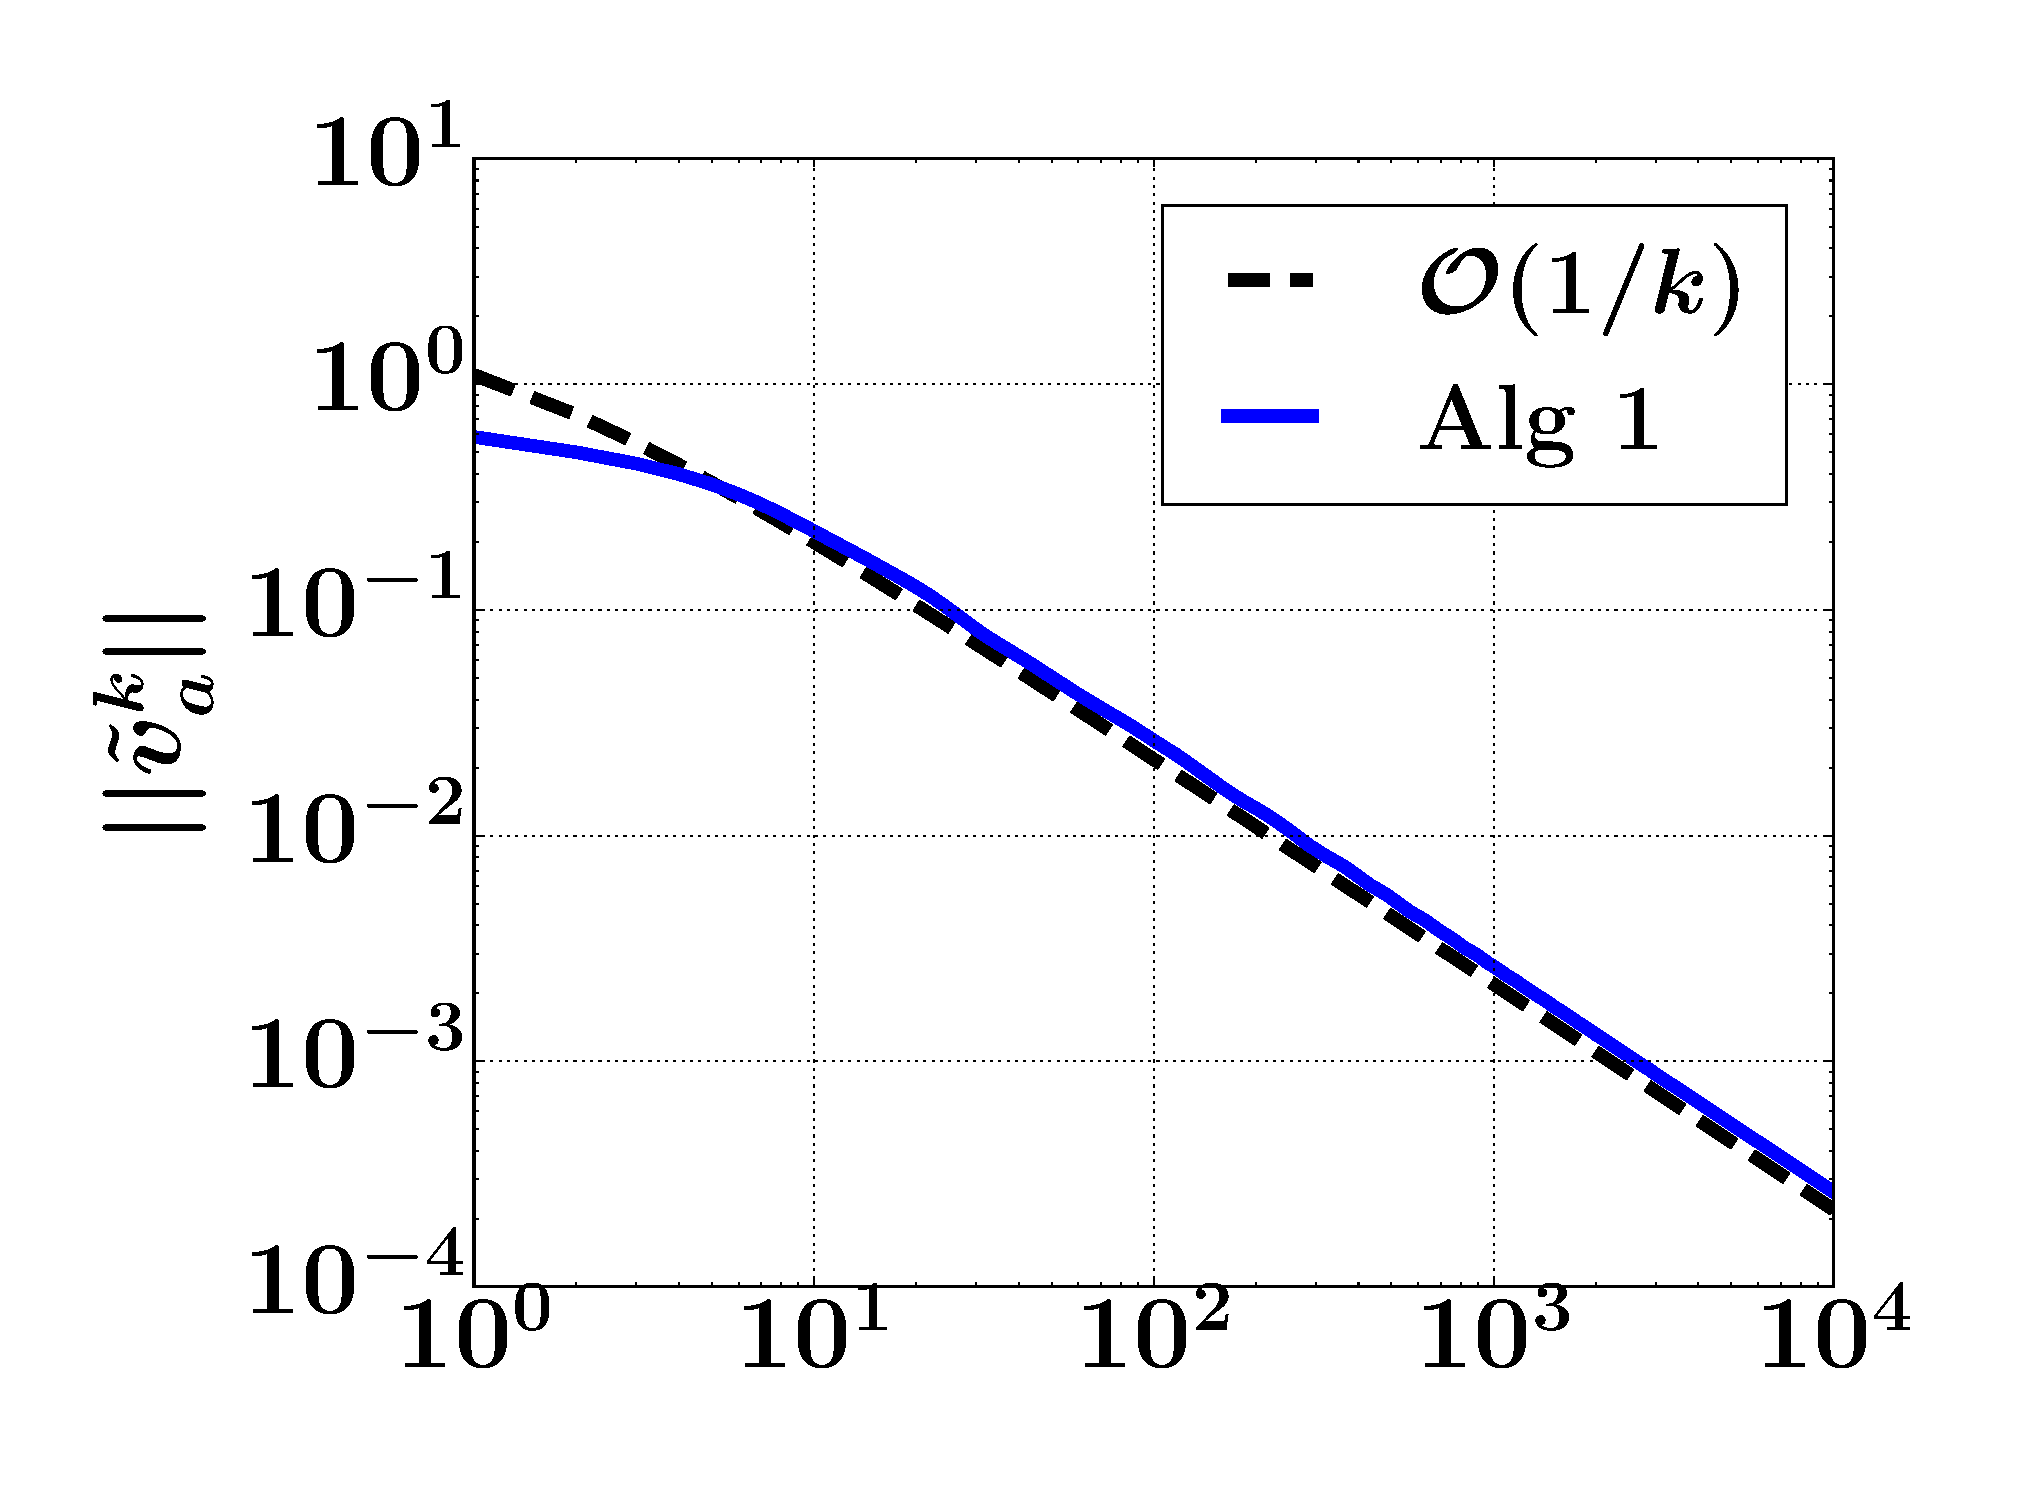
\includegraphics[width=.34\linewidth]{simplex_dgap.pdf}
  \hspace{-1em}
  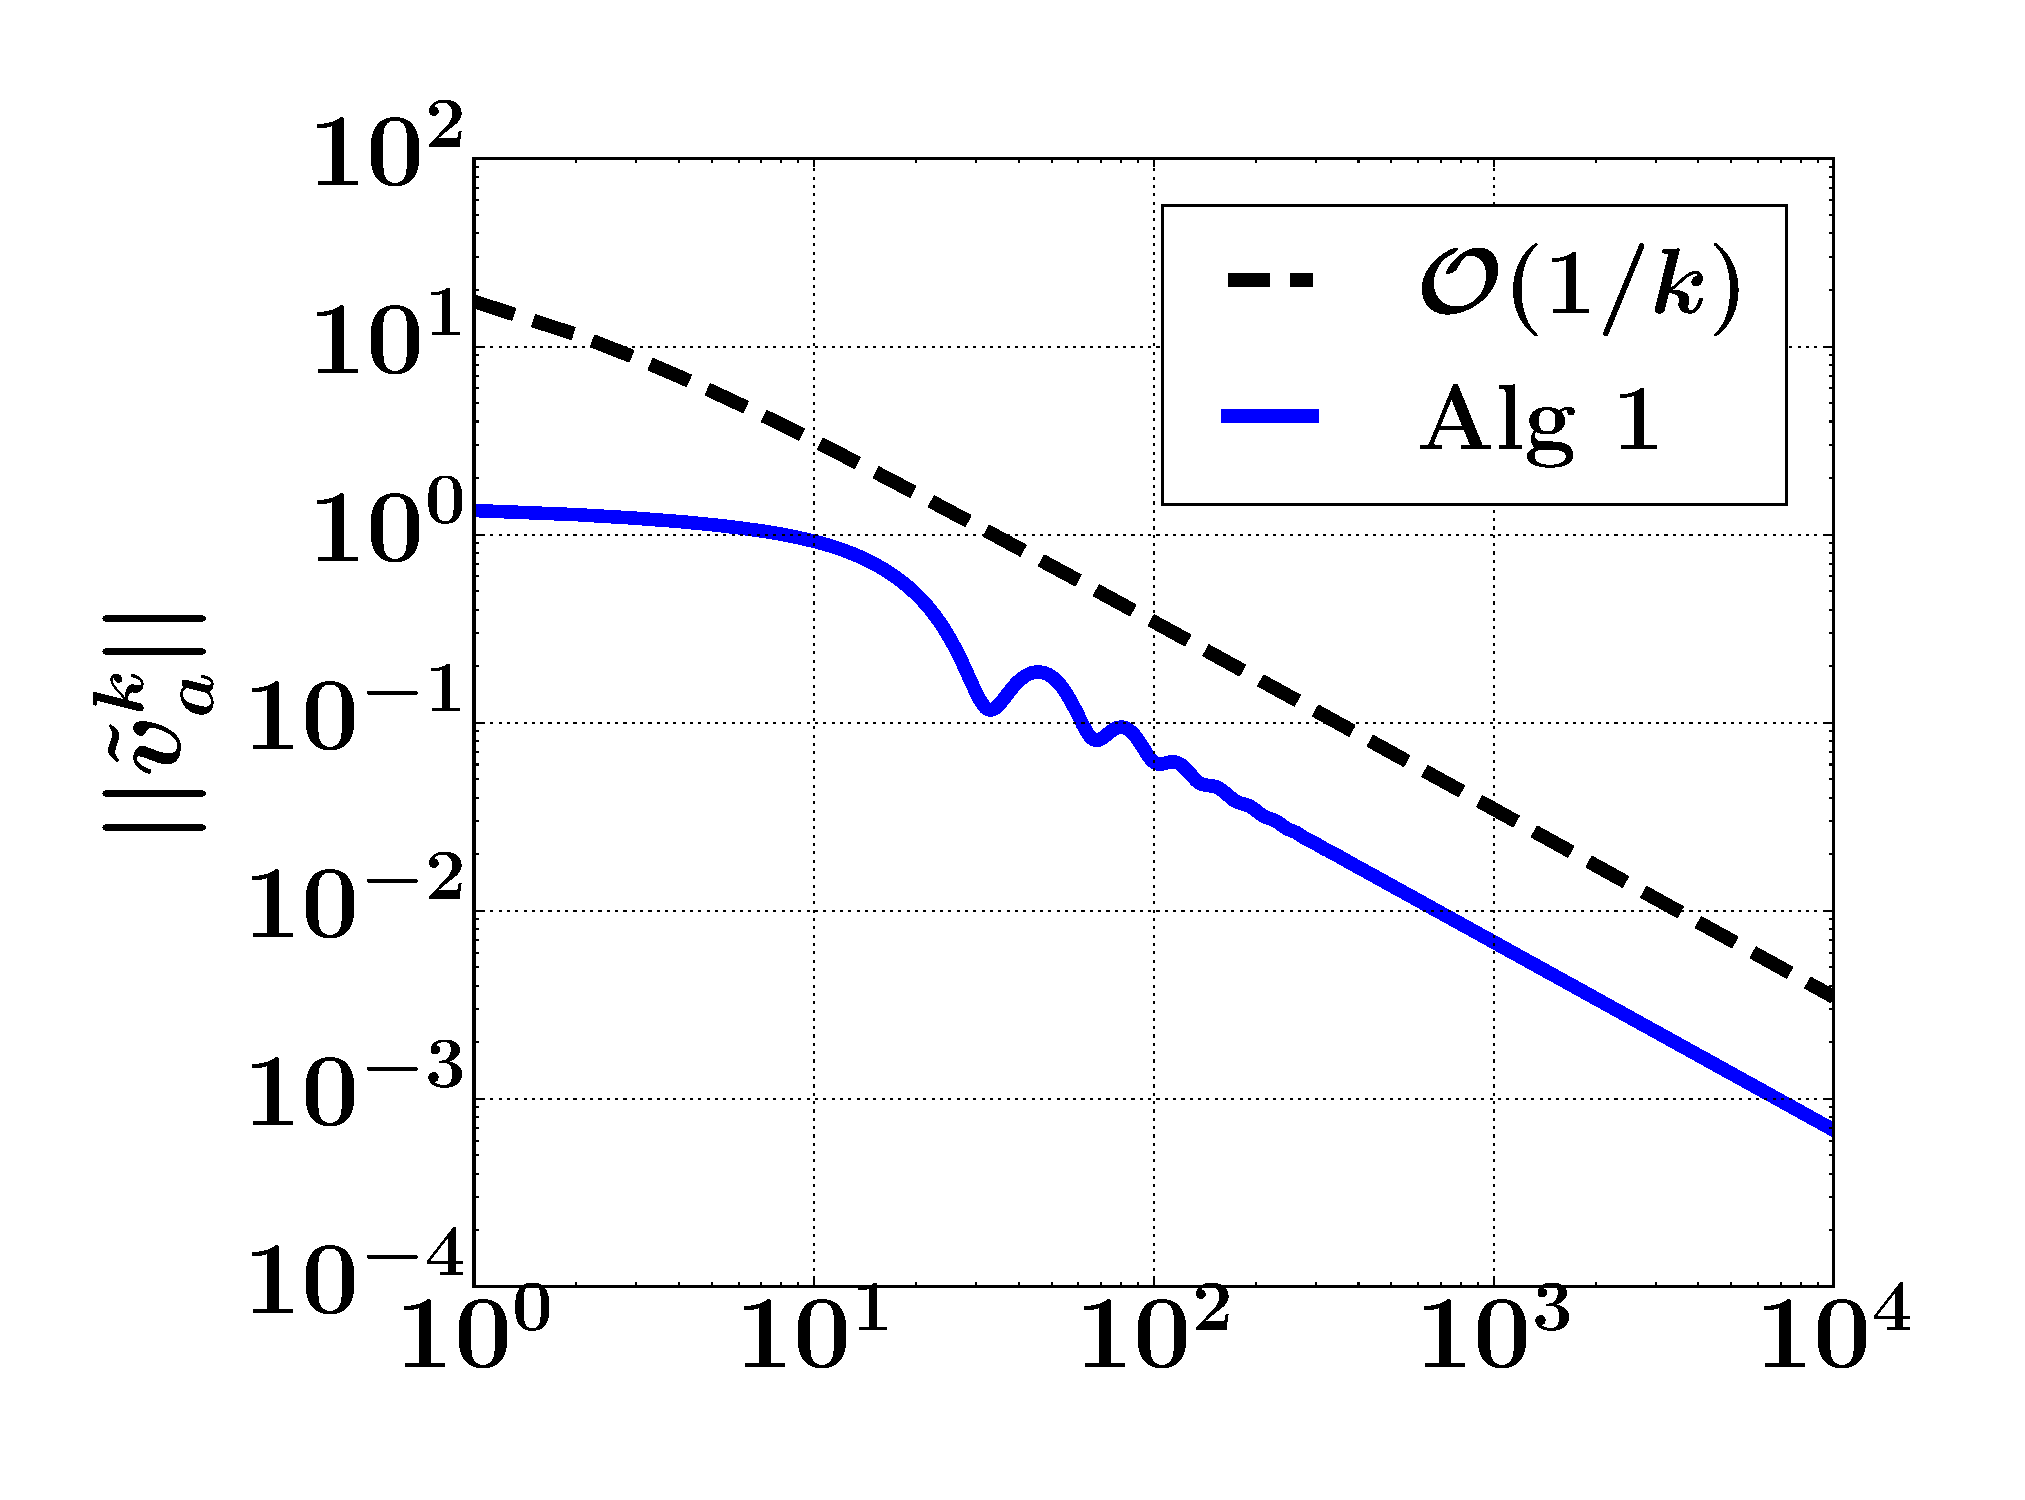
\includegraphics[width=.34\linewidth]{SimplifiedPoker_dgap.pdf}
  \hspace{-.8em}
  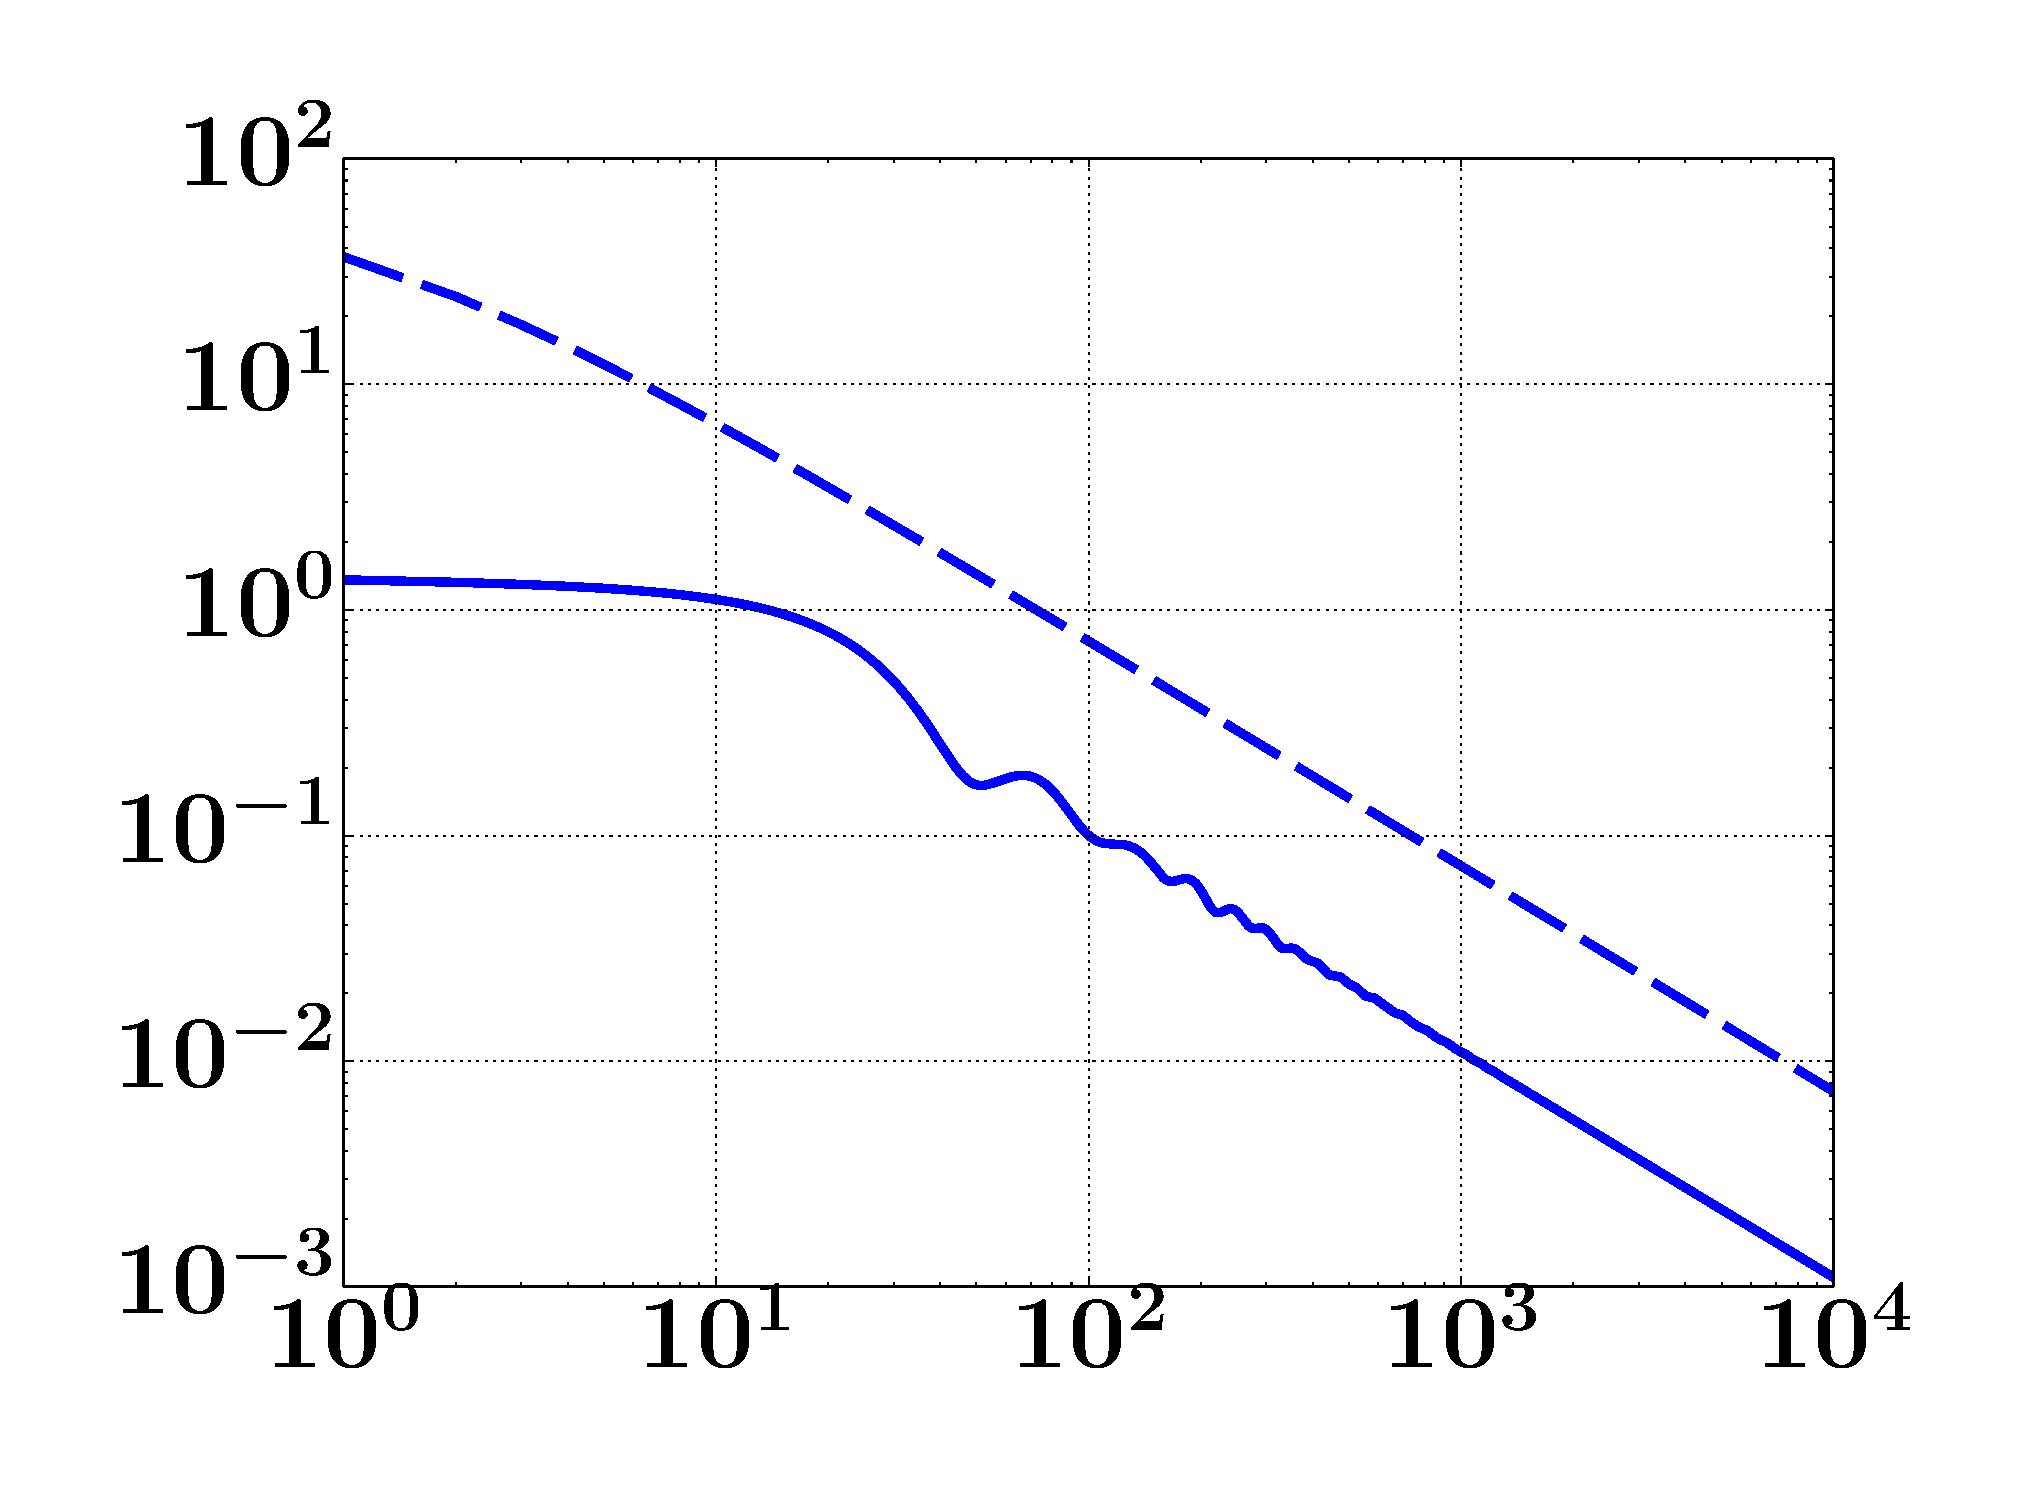
\includegraphics[width=.34\linewidth]{Kuhn3112_dgap.pdf}
  \hspace{-1.3em}
  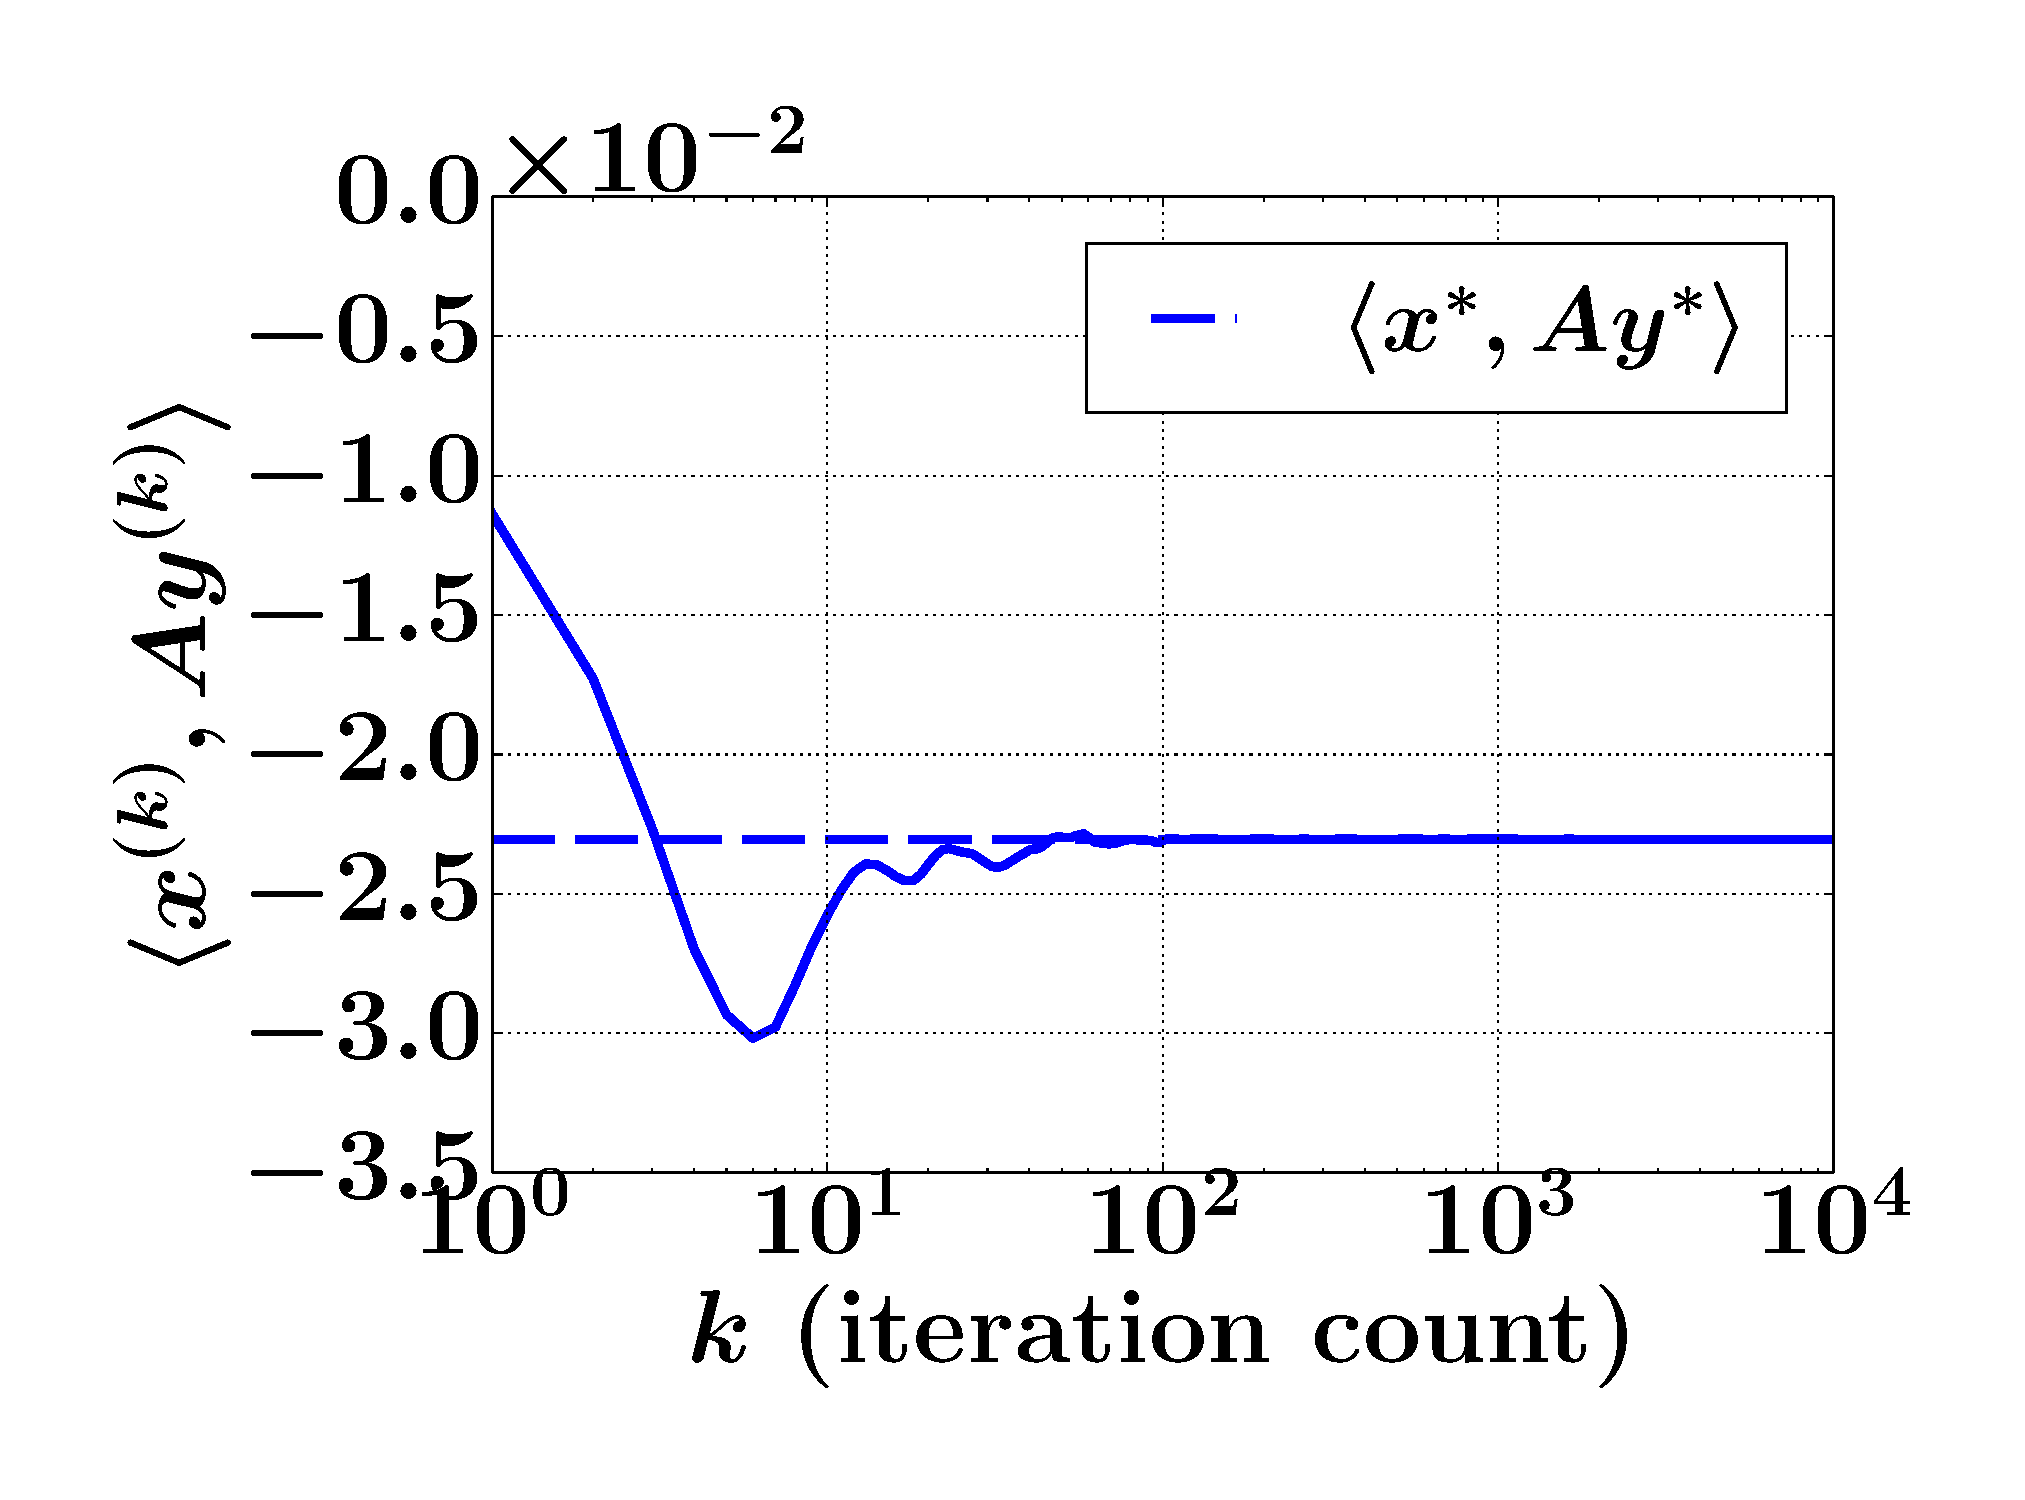
\includegraphics[width=.35\linewidth]{simplex_NE.pdf}
  \hspace{-.8em}
  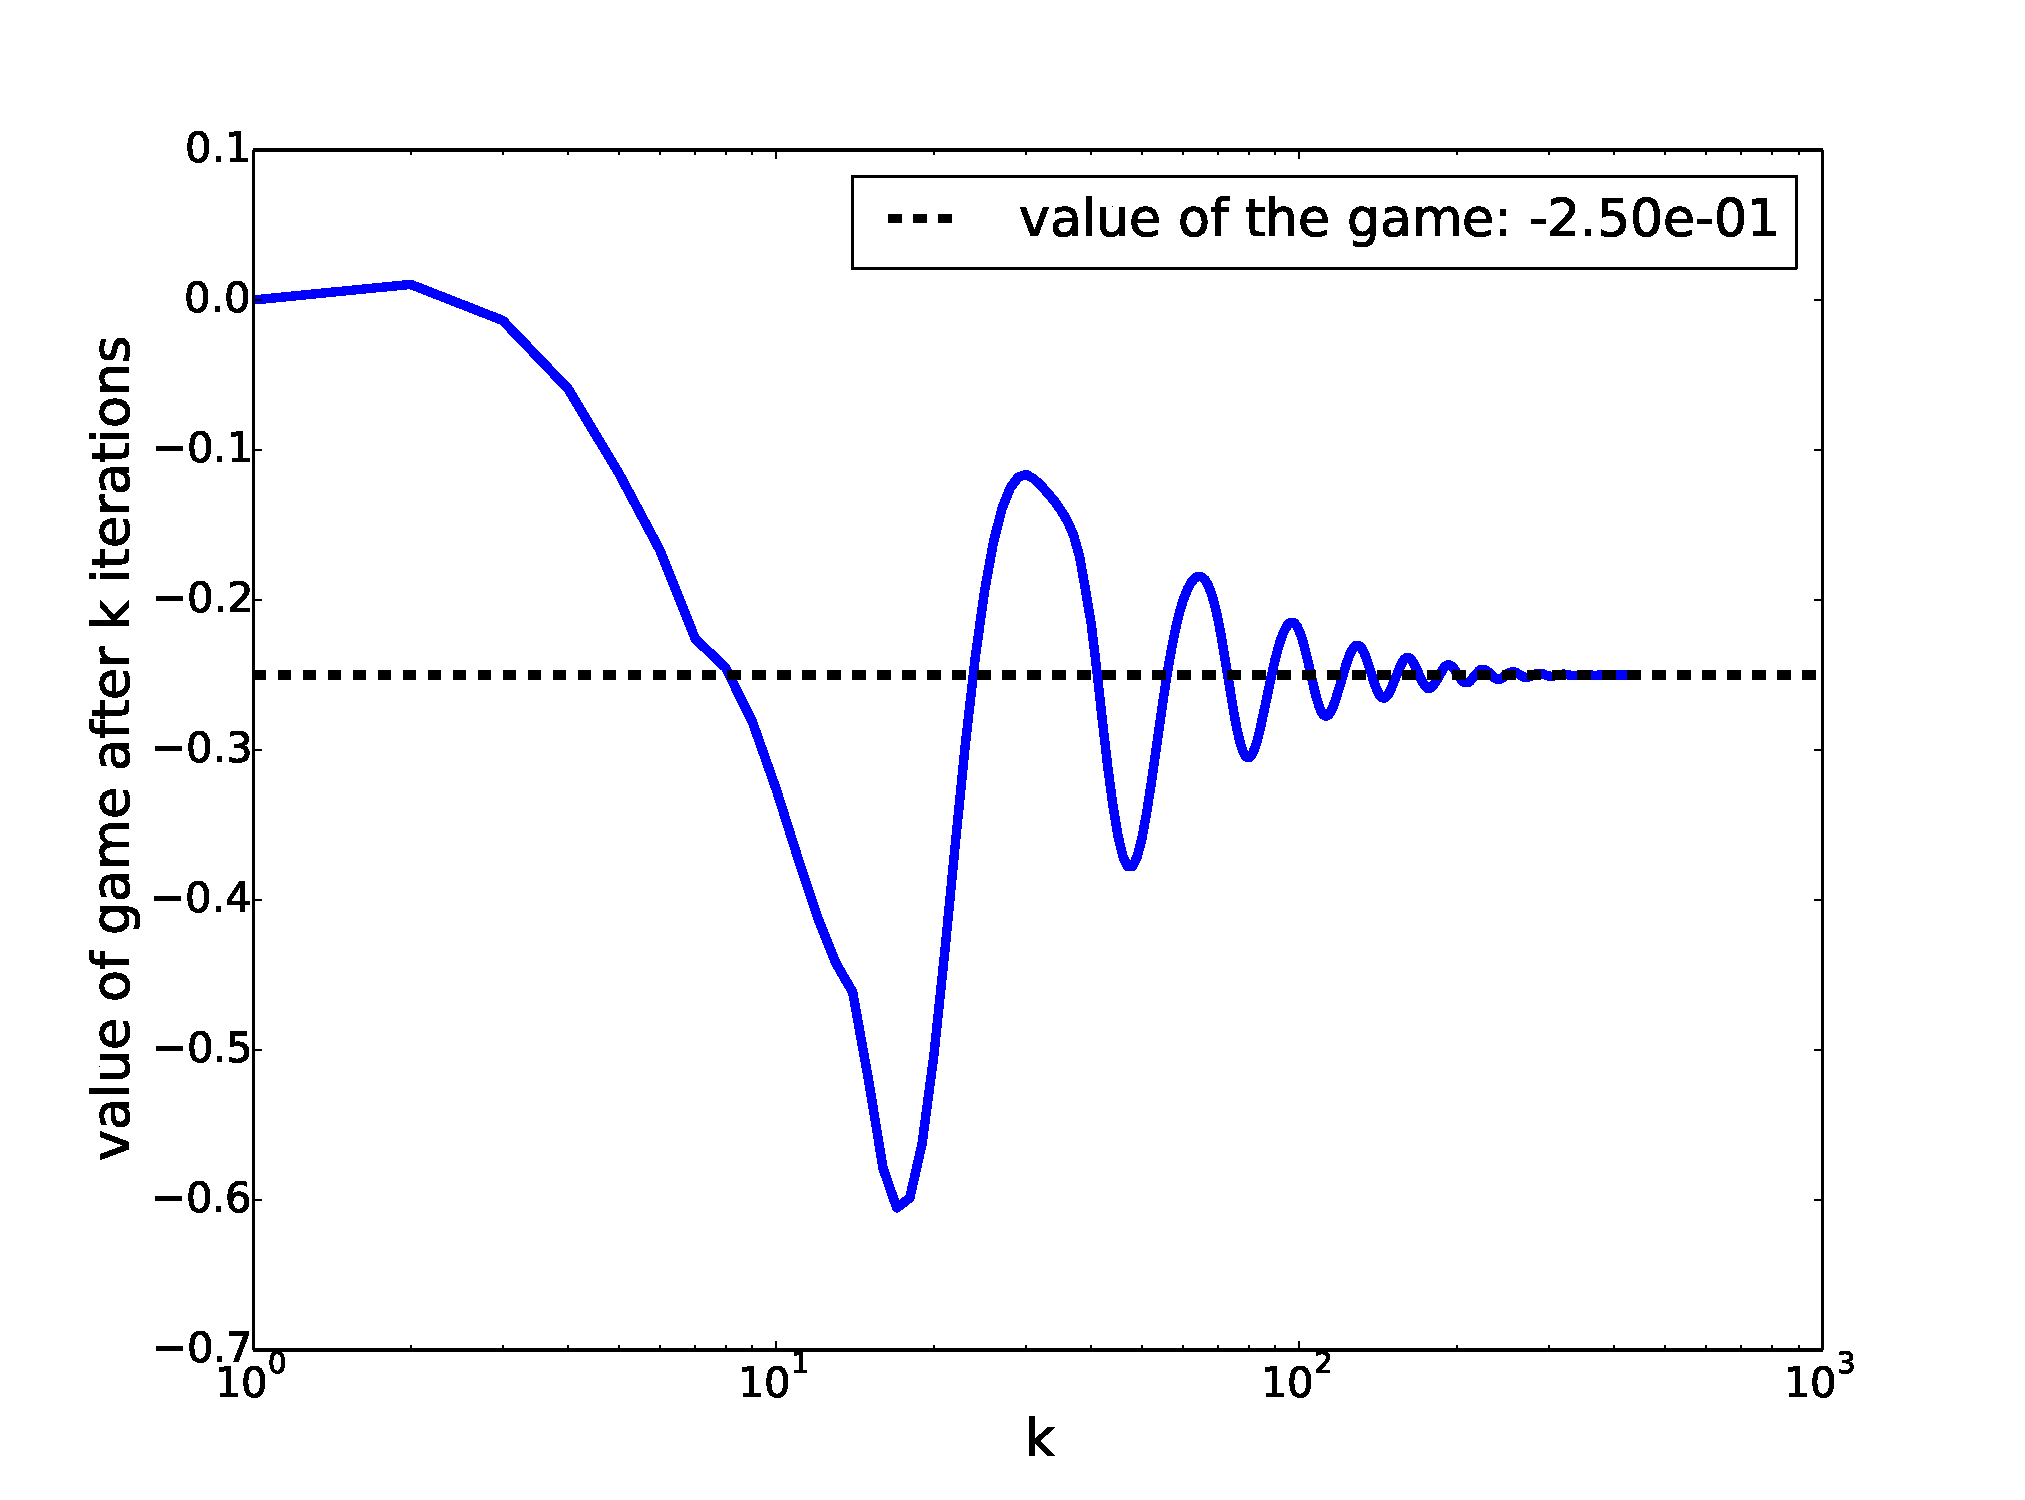
\includegraphics[width=.34\linewidth]{SimplifiedPoker_NE.pdf}
  \hspace{-1.3em}
  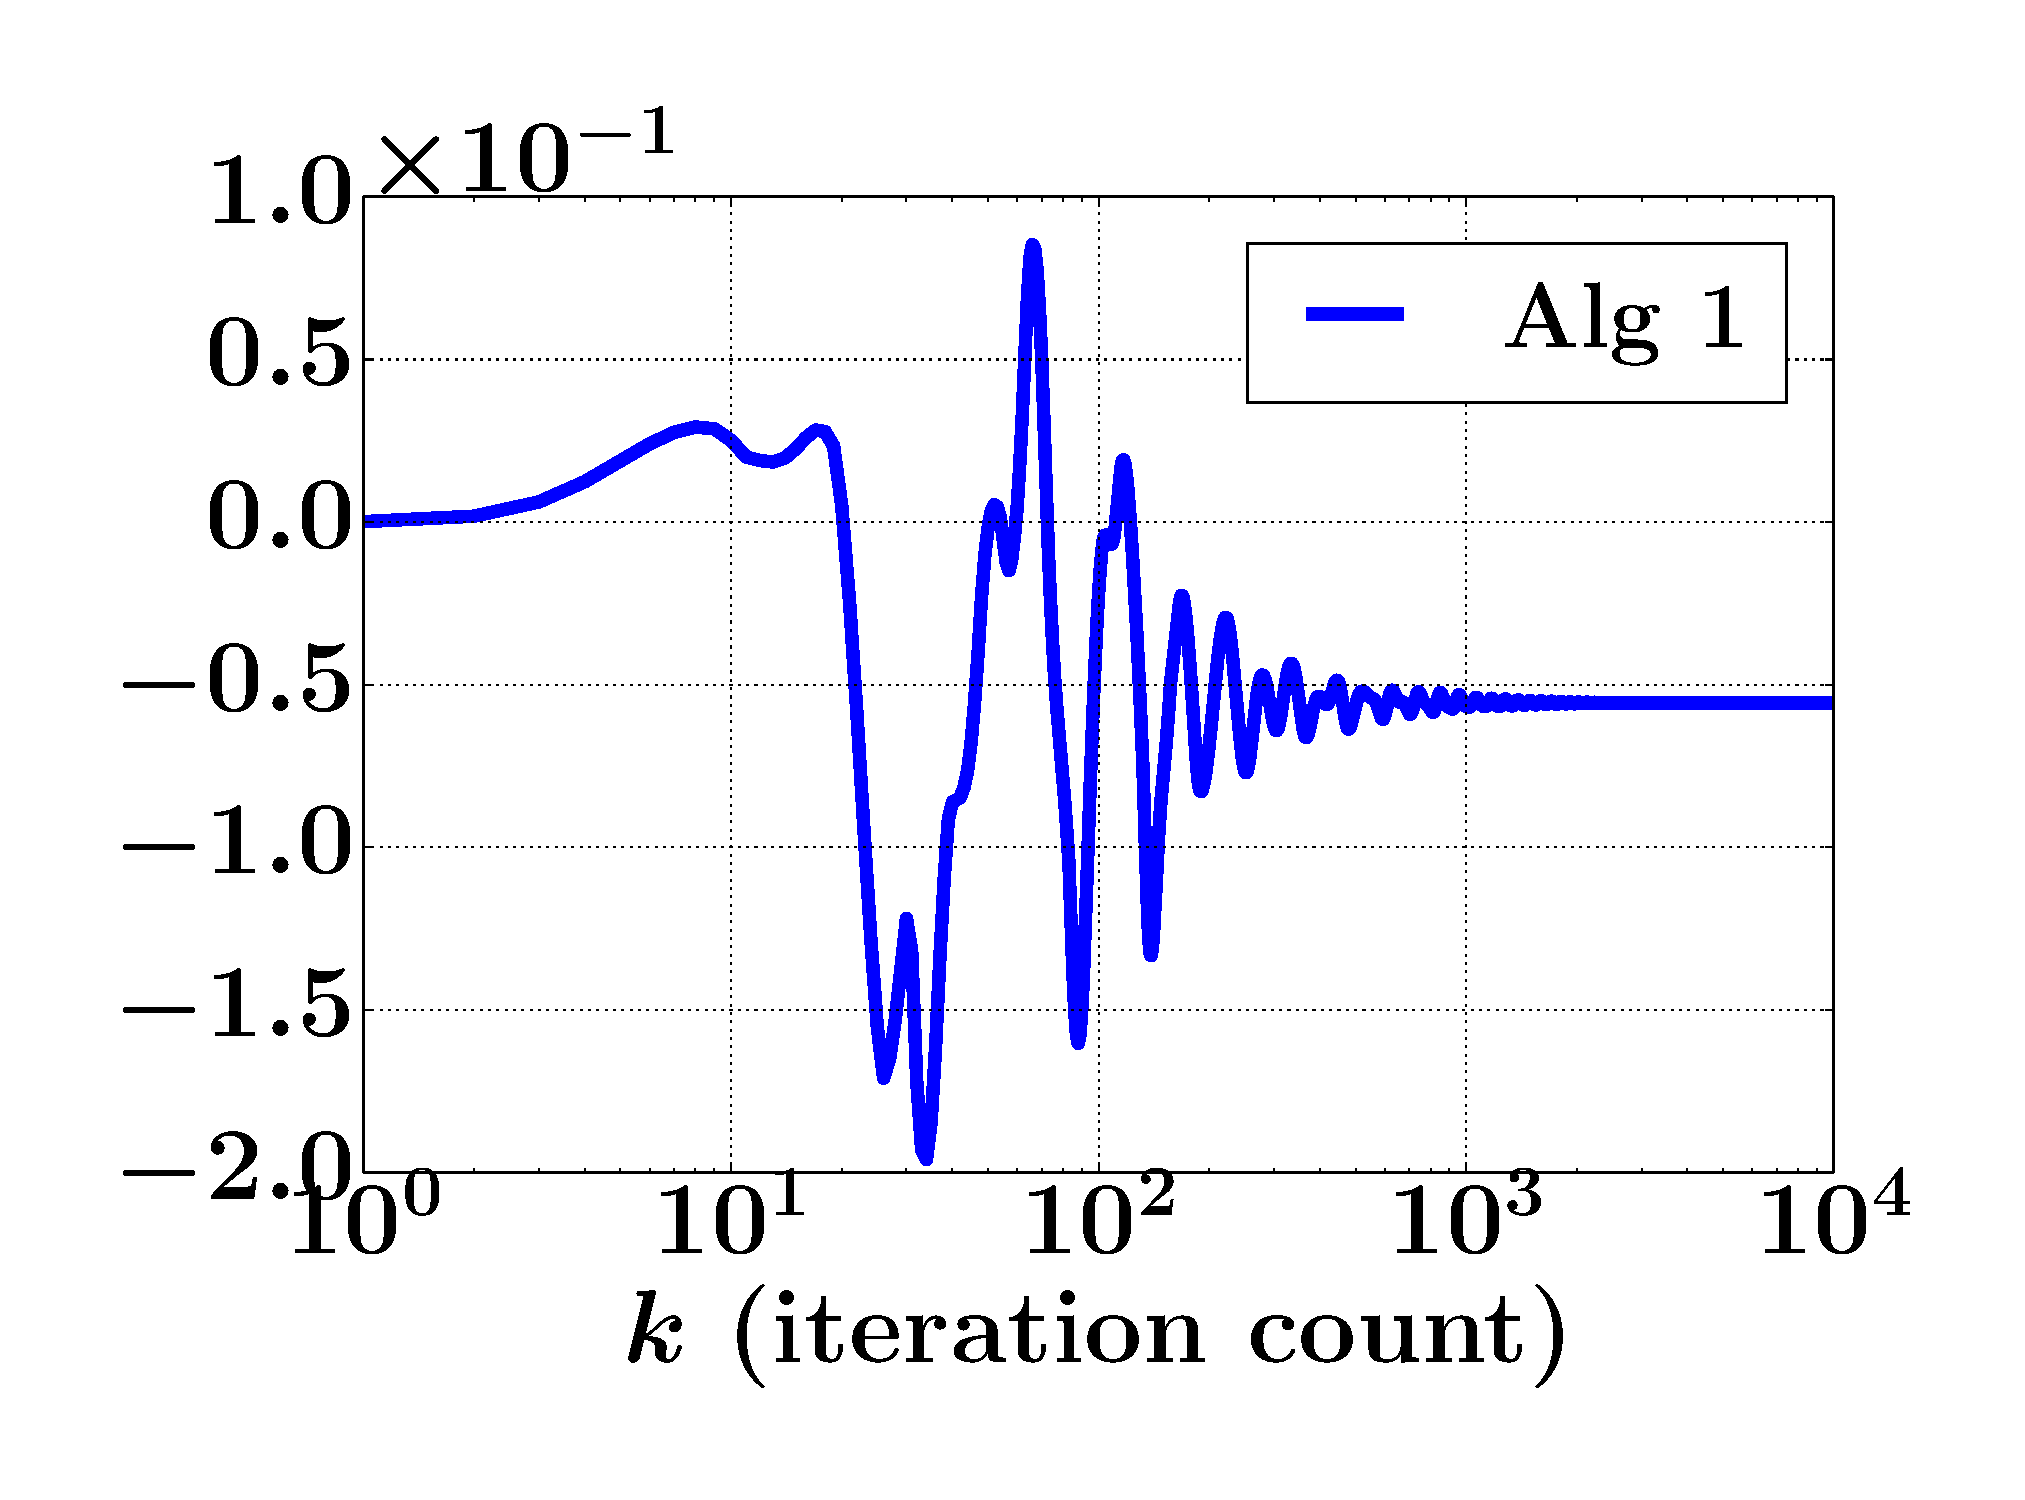
\includegraphics[width=.34\linewidth]{Kuhn3112_NE.pdf}
  \caption{Convergence curves of Algorithm
    \ref{Tab:algo_simplified}. \textbf{Left column}: Random $1000
    \times 1000$ matrix game on simplexes. \textbf{Middle column}:
    Simplified poker. \textbf{Right column}: Kuhn 3-card
    Poker. \textbf{Top row}: convergence in terms of ergodic
    duality-gap. \textbf{Bottom row}: Convergence in terms of value of
    game.}
  \label{Tab:dgap_curve}
\end{figure}

%% \begin{remark}
%% The results presented here are not meant to be benchmarks comparing
%% our algorithm to other algorithms, but should rather be seen as
%% proof-of-concept which experimentally  validates the rigorously
%% extablished results in section \ref{sec:algo}.
% \end{remark}

\subsection{Simulated game: matrix game on simplexes}
Any matrix $A \in \mathbb{R}^{n_1 \times n_2}$ specifies a
\textit{matrix game}. The strategy profile of player $k$ is a simplex;
this simplex can be written in the form \eqref{eq:polyhedron} by
taking $E_k := [1, 1, ..., 1] \in \mathbb{R}^{1 \times n_k}$ and $e_k
= 1$. Thus every matrix game on simplexes can be seen as a sequential
game. Now, as in \textbf{nesterov, c-p, etc.}, we generate a $1000
\times 1000$ random matrix whose entries are uniformly identically
distributed in the closed interval $[-1, 1]$. See Figure \ref{Tab:sim_dgap_curve}...

\subsection{Real-world game: Kuhn 3-card Poker}
The sequence-form representation of this simplified Poker variant
\cite{kuhn} is given by (not showing zero entries)\\

$E_1 = \left[\begin{array}{ccccccccccccc}
1 &   &   &   &   &   &   &   &   &   &   &   &  \\
-1 &   &   &   &   &   &   &   &   & 1 &   &   & 1\\
-1 & 1 &   &   & 1 &   &   &   &   &   &   &   &  \\
-1 &   &   &   &   & 1 &   &   & 1 &   &   &   &  \\
  & -1 & 1 & 1 &   &   &   &   &   &   &   &   &  \\
  &   &   &   &   & -1 & 1 & 1 &   &   &   &   &  \\
  &   &   &   &   &   &   &   &   & -1 & 1 & 1 &  
\end{array}\right] \in \mathbb{R}^{7 \times 13}$,
$E_2 = \left[\begin{array}{ccccccccccccc}
1 &   &   &   &   &   &   &   &   &   &   &   &  \\
-1 &   &   &   &   &   &   & 1 & 1 &   &   &   &  \\
-1 &   &   &   &   &   &   &   &   & 1 & 1 &   &  \\
-1 &   &   &   &   & 1 & 1 &   &   &   &   &   &  \\
-1 &   &   &   &   &   &   &   &   &   &   & 1 & 1\\
-1 & 1 & 1 &   &   &   &   &   &   &   &   &   &  \\
-1 &   &   & 1 & 1 &   &   &   &   &   &   &   &  
\end{array}\right] \in \mathbb{R}^{7 \times 13}$, $e_1 = e_2 = [1, 0,
  0, 0, 0, 0, 0]^T \in \mathbb{R}^7$, and $A =
\\\left[\begin{array}{ccccccccccccc}

  &   &   &   &   &   &   &   &   &   &   &   &  \\
  &   &   &   &   &   &   & -1 / 6 &   &   &   & -1 / 6 &  \\
  &   &   &   &   &   &   &   & -1 / 6 &   &   &   & -1 / 6\\
  &   &   &   &   &   &   &   & -1 / 3 &   &   &   & -1 / 3\\
  &   &   &   &   & 1 / 6 & -1 / 3 &   &   & 1 / 6 & -1 / 3 &   &  \\
  &   &   & 1 / 6 &   &   &   &   &   &   &   & -1 / 6 &  \\
  &   &   &   & -1 / 6 &   &   &   &   &   &   &   & -1 / 6\\
  &   &   &   & 1 / 3 &   &   &   &   &   &   &   & -1 / 3\\
  & 1 / 6 & 1 / 3 &   &   &   &   &   &   & 1 / 6 & -1 / 3 &   &  \\
  &   &   & 1 / 6 &   &   &   & 1 / 6 &   &   &   &   &  \\
  &   &   &   & -1 / 6 &   &   &   & -1 / 6 &   &   &   &  \\
  &   &   &   & 1 / 3 &   &   &   & 1 / 3 &   &   &   &  \\
  & 1 / 6 & 1 / 3 &   &   & 1 / 6 & 1 / 3 &   &   &   &   &   &  
\end{array}\right] \in \mathbb{R}^{13 \times 13}$.\\
The pair $(x^*, y^*) \in \mathbb{R}^{13} \times \mathbb{R}^{13}$ of
realization plans given by

\begin{eqnarray*}
  \begin{split}
    x^* &= [1, 0.759, 0.759, 0, 0.241, 1, 0.425, 0.575, 0, 0.275, 0,
      0.275, 0.725]^T,\\
    y^* &= [1, 1, 0, 0.667, 0.333, 0.667, 0.333, 1, 0, 0, 1, 0, 1]^T
    \end{split}
\end{eqnarray*}
is a Nash $10^{-4}$-equlibrium computed in 1500 iterations of
Algorithm  \ref{Tab:algo_simplified}. The convergence curves are shown
in Fig \ref{Tab:dgap_curve}. One easy checks that this equilibrium is
feasible. Indeed,

\begin{eqnarray*}
  \begin{split}
    E_1x^* - e_1 = [&4.76 \times 10^{-5}, -1.91 \times 10^{-5}, 5.67
      \times 10^{-5}, 8.23 \times 10^{-6}, 2.90 \times 10^{-5}, \\&
      -8.62 \times 10^{-7}, -1.96 \times 10^{-5}]^T
    \end{split}
\end{eqnarray*}
and

\begin{eqnarray*}
  \begin{split}
    E_2y^* - e_2 = [&-7.04 \times 10^{-7}, 2.27 \times 10^{-6}, -3.29
      \times 10^{-6}, -1.50 \times 10^{-6},\\
      &2.92 \times 10^{-6}, -4.97 \times 10^{-7}, -5.85 \times
      10^{-7}]^T
    \end{split}
\end{eqnarray*}
Finally, one checks that
\begin{eqnarray*}
  {x^*}^TAy^* = -0.055593685705289997,
\end{eqnarray*}
 which agrees to 4 d.p with the value of $-1 / 18$ computed
 analytically by H. W. Kuhn in his 1950 paper \cite{kuhn}. The
 evolution of the dual gap and the expected value of the game across
 iterations is shown in Figure \ref{Tab:dgap_curve}. These figures
 validate the theoritically established $\mathcal{O}(1/\epsilon)$
 convergence rate of the Algorithm.


\section{Conclusion}
Making use of the sequence-form representation
\cite{koller1992complexity,von1996efficient,vonequilibrium}, we have
deviced a primal-dual algorithm for computing Nash equilibria in
two-person zero-sum sequential games with imcomplete information (like
Texas Hold'em, etc.). Our algorithm is simple to implement, with a
very low constant cost per iteration, and enjoys a rigorous
convergence theory with a proven $\mathcal{O}(1/\epsilon)$ convergence
in terms of basic operations (matvec products, clipping, etc.), to a
Nash $\epsilon$-equilibrium of the game. The core of our contribution
(summarized in Theorems \ref{thm:pd} and \ref{thm:conv}) was to show
that a reformulation of the Nash equilibrium problem for sequential
games with imcomplete information lends the problem directly
accessible to primal-dual framework
\cite{chambolle2010,chambolle2014ergodic}.

Equilibrium problems are saddle-point convex-concave problems, and as
such a natural choice for an algorithm would be in the family of
primal-dual algorithms. The author believes such primal-dual schemes
will receive more attention in the algorithmic game theory community
in future.


\medskip \noindent
%% \paragraph{About the author:} I'm a first-year PhD student in Computer Science at Universit\'e de Parix XI. My thesis focuses on novel techniques for optimization on Lie groups (of diffeomorphisms), and other structured manifolds, the aim being to obtain better algorithms for nonlinear registration of fMRI brain images and enhance the charting of human functional connectomes.

\paragraph{Acknowledgments:} ...
\small
\bibliographystyle{splncs03}
\bibliography{bib}

\end{document}
